\documentclass[11pt,a4paper,11pt]{report}

\usepackage{amsfonts}
\usepackage{blindtext}
\usepackage{enumitem}
\usepackage{multicol}
\usepackage{geometry}
\usepackage{graphicx}
\geometry{hmargin=2.5cm,vmargin=2.0cm}
\usepackage[french]{babel}
\usepackage[T1]{fontenc}
\usepackage[utf8]{inputenc}
\usepackage{titlesec}
\usepackage{fancyhdr}
\usepackage{wrapfig}
\usepackage[amssymb]{SIunits}
\usepackage{amsmath}
\usepackage[final]{pdfpages}
\usepackage{bm}
\usepackage{array}
\usepackage{tabularx}
\usepackage[hyphens]{url} %pour retour à la ligne pour les liens
	\def\UrlBreaks{\do\.\do\@\do\\\do\/\do\!\do\_\do\|\do\;\do\>%
\do\]\do\)\do\,\do\?\do\'\do+\do\=\do\#\do\a\do\b\do\c\do\d\do\e\do\f\do\g\do\h\do\i\do\j\do\k\do\l\do\m\do\n\do\o\do\p\do\q\do\r\do\s\do\t\do\u\do\v\do\w\do\x\do\y\do\z%
\do\A\do\B\do\C\do\D\do\E\do\F\do\G\do\H\do\I\do\J\do\K\do\L\do\M\do\N\do\O\do\P\do\Q\do\R\do\S\do\T\do\U\do\V\do\W\do\X\do\Y\do\Z%
\do\1\do\2\do\3\do\4\do\5\do\6\do\7\do\8\do\9\do\%\do\=}%
\usepackage{lscape}
\usepackage{footnote}
\pagestyle{fancy}
\titleformat{\chapter}[hang]{\bf\huge}{\thechapter}{2pc}{}

\setcounter{secnumdepth}{3}
\setcounter{tocdepth}{3}


% FONCTIONS CREES POUR LES TABLES DE FIGURES ET LISTE DE TABLEAU

\let\pagebreakORIG\pagebreak
\let\clearpageORIG\clearpage
\let\cleardoublepageORIG\cleardoublepage
 
\ifx \removepagebreak \undefined
	\newcommand{\removepagebreak}{\renewcommand{\pagebreak}{}\renewcommand{\clearpage}{}\renewcommand{\cleardoublepage}{}}
\fi
 
\ifx \restorepagebreak \undefined
	\newcommand{\restorepagebreak}{\renewcommand{\pagebreak}{\pagebreakORIG}\renewcommand{\clearpage}{\clearpageORIG}\renewcommand{\cleardoublepage}{\cleardoublepageORIG}}
\fi

%%%%%%%%%%%%%%%%%%%%%%%%%%%%%%%%%%%%%%%%%%%%%%%%%%%%%%%%%%%%%%%%%%%%%%%%

\titlespacing{\chapter}{0pt}{*3}{*5}


\begin{document}

\fancyhead[L]{Rapport final}
\fancyhead[R]{\og Le Thermostat Intelligent \fg}
\renewcommand\thesection{\arabic{section}}

\begin{titlepage}

\newcommand{\HRule}{\rule{\linewidth}{0.6mm}} % Defines a new command for the horizontal lines, change thickness here

\center % Center everything on the page
 
%----------------------------------------------------------------------------------------
%	HEADING SECTIONS
%----------------------------------------------------------------------------------------
%\textsc{\LARGE Université Libre de Bruxelles}\\[1cm] % Name of your university/college

%----------------------------------------------------------------------------------------
%	LOGO SECTION
%----------------------------------------------------------------------------------------
\emph{} \\
\begin{minipage}{0.45\textwidth}
\begin{flushleft} 

\includegraphics[height=2cm] {images/logopolytech.jpg}\\
\end{flushleft}
\end{minipage}
~
\begin{minipage}{0.45\textwidth}
\begin{flushright} 

\includegraphics[height=2cm] {images/logoulb.jpg}\\
\end{flushright}
\end{minipage}\\[1.5cm]


%
\includegraphics{Logo}\\[1cm] % Include a department/university logo - this will require the graphicx package
 
%----------------------------------------------------------------------------------------

\textsc{\Large Rapport final}\\% Major heading such as course name
\emph{} \\
\textsc{\large TRAN-H-201}\\[1.5cm] % Minor heading such as course title

%----------------------------------------------------------------------------------------
%	TITLE SECTION
%----------------------------------------------------------------------------------------

\HRule \\[1cm]
{ \huge \bfseries \og Le Thermostat Intelligent \fg}\\[1cm] % Title of your document
\HRule \\[2cm]
 
%----------------------------------------------------------------------------------------
%	AUTHOR SECTION
%----------------------------------------------------------------------------------------


\begin{minipage}[]{0.4\textwidth}
    \begin{center}
        {\large \textit{Étudiants}:\vspace*{0.5cm} \\
        \textsc{Amzur} Soufiane\\
        \textsc{Daubry} Wilson\\
        \textsc{Sercu} Stéphane\\
        \textsc{Verstraeten} Denis\\ 
        }
    \end{center}
\end{minipage}%
%
\begin{minipage}[]{0.4\textwidth}
    \begin{center}
        {\large \textit{Superviseur}:\vspace*{0.5cm} \\ 
        \textsc{Eppe} Stefan}\\
        \vspace*{0.5cm}
        {\large \textit{Lecteur}:\vspace*{0.5cm} \\ 
        \textsc{Vermeir} Aurélien }\\
    \end{center}    
\end{minipage}

\emph{} \\
\emph{} \\
\emph{} \\
\emph{} \\
\emph{} \\
\emph{} \\
\emph{} \\
\emph{} \\
\emph{} \\
\emph{} \\
\emph{} \\
\emph{} \\
\emph{} \\
\emph{} \\
\emph{} \\
\emph{} \\
\emph{} \\
\emph{} \\



\iffalse
\begin{minipage}{0.4cm\textwidth}
\begin{flushleft} \large
\emph{Étudiants:}\\
\emph{} \\
\textsc{Amzur} Soufiane\\
\textsc{Daubry} Wilson\\
\textsc{Sercu} Stéphane\\
\textsc{Verstraeten} Denis\\ 
\end{flushleft}
\end{minipage}

~

\begin{minipage}{0.4\textwidth}
\begin{flushright} \large
\emph{Superviseur:}\\
\emph{} \\
\textsc{Eppe} Stefan\\
%\vspace{2.0cm}
\hspace{3.0cm}
\emph{} \\
\emph{} \\
\emph{} \\
\end{flushright}
\end{minipage}
\fi



\iffalse
\begin{minipage}{0.4\textwidth}
\begin{flushright} \large
\emph{} \\
\emph{} \\ %Ca m'a permis de aligner les 2 mini-pages
\emph{} \\
\emph{} \\
\emph{} \\
\emph{Superviseur:} \\
\emph{} \\
\textsc{Eppe} Stefan \\ % Supervisor's Name
\vspace{2.0cm}
\emph{Lecteur: } \\
\emph{} \\
\textsc{Vermeir} Aurélien \\ % Supervisor's Name
\end{flushright}
\end{minipage}\\[4cm]% Plus il est grand et plus la date "Décembre" descend en bas
\fi
% If you don't want a supervisor, uncomment the two lines below and remove the section above
%\Large \emph{Author:}\\
%John \textsc{Smith}\\[3cm] % Your name

%----------------------------------------------------------------------------------------
%	DATE SECTION
%----------------------------------------------------------------------------------------

{\large 14 Mars 2016}\\[0cm] % Date, change the \today to a set date if you want to be precise

\vfill % Fill the rest of the page with whitespace

\end{titlepage}

%----------------------------------------------------------------------------------------
%	ABSTRACT
%----------------------------------------------------------------------------------------

\chapter*{Abstract}
%il faut trouver un meilleur titre of course :p
\textbf{“Realisation of a Smart Thermostat using Raspberry Pi and Arduino Nano”,
by \textsc{Amzur} Soufiane, \textsc{Daubry} Wilson, \textsc{Sercu} Stéphane and \textsc{Verstraeten} Denis, Université Libre de Bruxelles, 2015-2016.}
\vspace{0.2cm}\\
The purpose of this project is to design a smart thermostat. The principle is simple: a Raspberry Pi 2 Model B with Python and a Wifi antenna communicates with \og thin thermostats \fg thanks to the http protocol. These \og thin thermostats\fg are microcontrollers supplied with a thermistor, a presence sensor and a module Wifi. Data collected can be gathered and stored in a SQLite database. As a first step, a simple reactive control has to be implemented in the central server. It consists of to open or to close thermostatic valve depending on whether it is too cold or too hot. A smarter and more predictive control algorithm will be then implemented using databases in order to learn the habits and the preferences of users. At the end, it will be necessary to set up a rigourous test protocol. The aim of those tests is to ensure the quality of the system as well quantitatively as qualitatively.\newline
 
\textit{Key words:  thermostat, microcontroller, smart, databases, server, data mining, machine learning}\newline
[Word limit: 160]
\newline

\textbf{“Realisation d'un thermostat intelligent avec un Arduino et un Raspberry Pi”,
par \textsc{Amzur} Soufiane, \textsc{Daubry} Wilson, \textsc{Sercu} Stéphane et \textsc{Verstraeten} Denis, Université Libre de Bruxelles, 2015-2016.}
\vspace{0.2cm}\\
Le but de ce projet est de créer un système de thermostats intelligents. Un thermostat central doit être implémenté en Python sur un Raspberry Pi 2B équipé d'une antenne Wi-Fi avec laquelle il communique suivant le protocole HTTP avec les \og thin thermostats \fg ~. Ces derniers sont composés d'un micro-contrôleur Arduino Nano V2, d'un capteur de présence, d'une thermistance et d'un module Wi-Fi, le tout monté sur une BreadBord. Un environnement y est également connecté, lequel possède une vanne de chauffage et alimente l'Arduino. Ils servent uniquement à prendre des mesures stockées par le Rapsberry dans une base de données implémentée en SQLite et à actualiser la valeur de la vanne. Un algorithme de contrôle réactif est premièrement intégré, suivant le principe du \og ON/OFF \fg. Il est suivi d'un algorithme intelligent et prédictif se basant sur le \og vécu \fg du thermostat et les habitudes de l'utilisateur, il se veut également écologique en minimisant les oscillations de température à l'aide d'un régulateur PID. Des stratégies de tests et une validation du modèle devront être mis en place dans l'objectif de dégager des indicateurs objectifs de performance.\newline

\textit{Mots-clés:  thermostat, microcontrôleur, intelligence, base de données, serveur}\newline
[Limite de mots: 188]

\newpage

%----------------------------------------------------------------------------------------
%	TABLE DES MATIERES
%----------------------------------------------------------------------------------------

\renewcommand{\contentsname}{Table des matières}
\tableofcontents
\listoffigures  % table des figures
\removepagebreak
\listoftables 
\restorepagebreak

%---------------------------------------------------------------------------------------
%	INTRODUCTION
%----------------------------------------------------------------------------------------
\renewcommand{\baselinestretch}{1.5}

\chapter{Introduction} % Modifié par Stéphane: adaptation pour le 2ème Q.

Actuellement, il y a une très forte augmentation de l’offre et de la demande d’objets connectés ou intelligents, car le désir d’une utilisation simplifiée et automatisée est grandissant. C’est dans cette optique que s’inscrit ce projet multidisciplinaire orienté vers l’informatique : \og Thermostat intelligent \fg. En effet, le dispositif à concevoir se doit d'être autonome, doté d’un modèle de prédiction personnel, adapté aux habitudes de l’utilisateur et minimisant la consommation énergétique en évitant les oscillations de température.\\
% TODO: "D'autre part, la climatisation des intérieurs => une des plus grosse épense énergique

Le projet d’année des étudiants en bloc deux de l’école polytechnique consiste en la réalisation d’un thermostat intelligent. Ce dernier sera composé de deux types de périphériques, une unité centrale qui sera un Raspberry Pi 2 et des \og Remote Devices \fg ~qui seront des Arduinos Nano.\\

Dans ce rapport, la conception globale du thermostat est abordée en premier. L'implémentation en language Arduino\footnote{Sketch} (proche du C) et son câblage suit, avant de passer au thermostat central. Le développement des outils indispensables à son fonctionnement, tels qu'un serveur, une base de données, un processus de récolte de données et un régulateur en boucle fermée est d'abord abordée. Ensuite les différent modèles prédictifs, se basant sur les précédents outils et servant l'intelligence du thermostat ainsi que leur implémentation sont présentés. L'intelligence du code en elle même suivra. Cette partie étant composée de la prédiction de présence et du temps de chauffe. Une validation de ces modèles afin vérifier que ces dispositifs sont fonctionnels et efficaces est ensuite explicitée, avant de poursuivre avec le fonctionnement de groupe. Cette  partie détaille la manière dont le travail à été réparti et organisé. Des perspectives d'évolutions sont également envisagées, celles-ci listant principalement des fonctionnalités et des amélioration qu'il serait intéressant d'ajouter au prototype.\\

Les notations propres au langage UML 2.0 sont utilisées. Les conventions d'association, d'agrégation, d'héritage, de public, privé sont conservées. Les schémas de comportement et d'initialisation, correspondent aux diagrammes d'interaction du langage. Dans ces derniers, les cadres ne respectent pas le formalisme usité. Les formes des cadres principalement, ces diagrammes ayant pour but principal d'assurer a compréhension du fonctionnement du thermostat, ils ne se veulent pas extrêmement rigoureux.\\

Il est également important de mentionner que ce rapport ne fait pas état des codes exacts qui se trouvent dans le dépôt GIT, il expose la structure envisagée. En effet, suite à des problèmes liés au module Wi-Fi de l'Arduino indépendants de notre volonté, la cadence de travail dû être fortement ralentie. Durant plusieurs semaines, la communication entre le thermostat central et les Remotes Devices fut impossible. Les tests ne furent plus possibles, les vérifications de l'avancement du travail non plus. C'est donc pour cela que certains tests ne sont pas concluant. Des alternatives durent donc être trouvées, mais il ne fut pas possible d'en déterminer pour tout.\\

\newpage
%--------------------------------------------------------------------------------------
%	CONCEPTION
%--------------------------------------------------------------------------------------

\chapter{Conception}

Afin de commencer sur une bonne base et d'offrir une vue globale du projet, un diagramme (présenté en Annexe \ref{dia_complet}) a été construit. Le but premier de celui-ci est d'offrir une vue globale et commune du développement à tous ses contributeurs. Cela permet principalement le partage efficace des différentes parties à développer entre les participants. Le rassemblement de tous les modules est également grandement simplifié. En effet, il est beaucoup plus facile d'assembler des parties du projet qui ont été construites en gardant en tête la place qu'elles occupent dans son ensemble et la façon dont elles sont sensées communiquer les unes avec les autres.\\
% TODO: terme subjectif "grandement", "beaucoup", .. à supprimé? remplacer?

%to do : référence annexe et figure à rajouter

En plus de tous ces avantages pratiques, ce diagramme a un grand pouvoir documentaire puisqu'il offre une vision synthétique et schématique de l'ensemble du projet.
Il n'a pas été construit en une fois. En effet, il a été complété et corrigé lors de l'avancée du développement en fonction des discussions menées concernant certains problèmes et choix qui ont dû être opérés.
Le diagramme est explicité et décrit plus en détails dans le reste du rapport puisque chacune des parties principales du projet est détaillée sur cette base.



\newpage
%--------------------------------------------------------------------------------------
%	ARDUINO
%--------------------------------------------------------------------------------------

\chapter{Thermostats auxiliaires}

\section{Hardware}

D’un point de vue hardware, le montage de l’Arduino Nano est réalisé sur une BreadBord. Les éléments ayant été intégrés à ce câblage sont :\newline
\begin{itemize}
	\item Un Arduino Nano V2 \cite{ar1} \newline
    \item Une thermistance et une résistance de 10k$\ohm$ \cite{datash} \newline
	\item Un capteur de présence infrarouge (PIR\footnote{Passive Infrared} sensor) \cite{ar3} \newline
	\item Un module Wi-Fi ESP-8266 \cite{ar4} \newline
	\item Une vanne thermostatique \newline
\end{itemize}

Ces quatre composants doivent être alimentés et leur signaux de retour captés par le microcontrôleur. Leurs spécificités d’utilisation indiquées dans leur datasheet respective sont prises en compte afin d’éviter que le matériel ne soit endommagé. Ils sont donc branchés suivant la logique suivante :\\

\begin{figure}[h]
 \begin{center}
  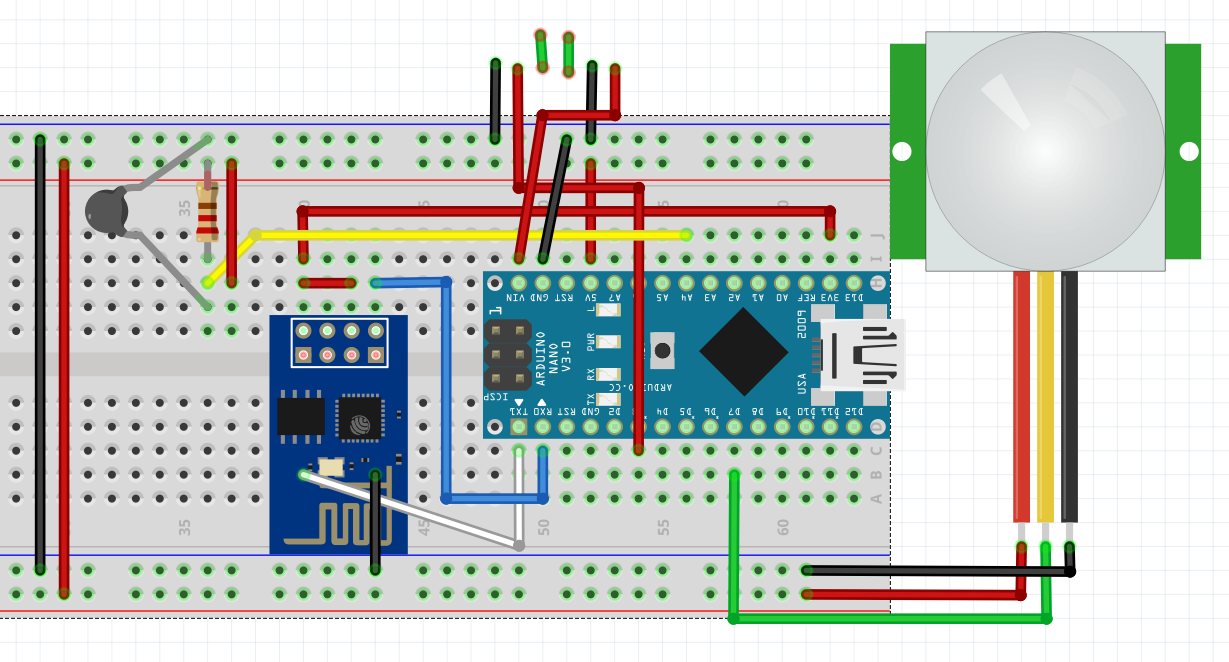
\includegraphics[width=0.6\linewidth]{images/cablage.png}
  \caption{Câblage du microcontrôleur}
  \label{arduino_cablage}
 \end{center}
\end{figure}

	Le détecteur de présence est muni de 3 câbles, un servant d’alimentation permettant de recevoir la tension de 5V, un autre étant la terre du circuit et le dernier devant être relié à une pin numérique afin de lire les données fournies par le détecteur. La pin numérique choisie est la pin D7. Ce choix est purement arbitraire, la seule obligation étant que l'entrée soit digitale.\\

	La thermistance nécessite également une tension d’entrée de 5V, celle-ci doit au préalable passer dans une résistance de 10k$\ohm$ branchée en série afin que la Loi d'Ohm puisse lui être appliquée. Elle est finalement reliée à la masse. Une lecture analogique du capteur est effectuée au moyen d'un câble reliant la pin A4 à la tension qui entre dans la thermistance.\\

Le branchement de module Wi-Fi est un petit peu plus complexe. D’abord, contrairement aux autres composants, il est connecté à une source d’alimentation de 3.3V délivrée par le micro-contrôleur. Cette tension doit être dirigée vers les pins \og VCC \fg ~et \og CH\_PD \fg ~du module Wi-Fi. Comme tous les autres composants, sa borne \og Ground \fg ~est connectée à la masse. Notons enfin la présence de 2 câbles indispensables qui assurent la communication entre l'Arduino et le module Wi-Fi, ce sont les câbles qui relient respectivement les bornes \og Rx \fg ~et \og Tx \fg ~du premier aux bornes \og Tx \fg ~et \og Rx \fg ~du second.\\

Enfin, il est à noter que l'Arduino est alimenté par un environnement physique grâce aux pin $V_{in}$ et $Gnd$. Ce premier \og renvoie \fg cette alimentation au travers de sa sortie 5V. L'Arduino peut également transmettre des ordres d'ouverture ou de fermeture partielle de la vanne au travers de la pin D3 directement reliée à l'environnement.\\

Les six fils isolés donnant l'impression de n'être branchés à rien sont en fait connectés à l'environnement. De droite à gauche se situent la masse de la vanne, son actuateur, deux câbles symbolisant une thermistance présente sur l'environnement, la masse de l'Arduino et son alimentation.\\

\section{Software}

D’un point de vue du software, il faut que le microcontrôleur soit capable de lire les informations des différents capteurs mais qu’il puisse aussi générer à partir de cette lecture un type d'information exploitable. Une structure de base de code a été fournie. Elle est axée sur une optimisation de la mémoire, assez réduite, de l’Arduino et elle est complétée par les fonctions nécessaires.\\ 

Le PIR n’envoie que deux types de signaux, à savoir présence ou pas de présence. Ceux-ci auront la forme de HIGH ou LOW, respectivement. Ils seront convertis en booléens afin d'être plus facilement manipulables par le serveur.\\

Quant à la valve thermostatique, une variable globale contenant la valeur de son ouverture est stockée dans le code. Dès lors, lorsque qu'un ordre d'actualisation est reçu, la tension correspondante est envoyée et la valeur de la variable est mise à jour. Lorsqu'on souhaite consulter la valeur de l'ouverture, la variable est renvoyée. De cette façon, il est possible d'effectuer une lecture sans nécessiter de câblages supplémentaires.\\

Pour la mesure de la température, le calcul est un peu plus complexe. D’abord, ce qui sort du senseur est une valeur analogique comprise entre 0 et 1023 qui représente la différence de potentiel aux bornes de la thermistance. Elle dépend bien entendu de la température du milieu. Dans l'état actuel des choses, une valeur de 5 $\volt$ est utilisée dans la relation de conversion. Il a toutefois été envisagé d'effectuer une lecture analogique de cette tension et d'injecter la valeur trouvée dans l'expression afin qu'aucun biais sur la température n'apparaisse, ceci rendant le dispositif indépendant de la qualité de la source électrique qui l'alimente\footnote{Par exemple, lorsque l'Arduino est alimenté par un port USB, il ne délivre plus que 4.64 $\volt$.}. \\

Une fois la tension aux bornes de la thermistance connue, on peut déterminer sa résistance en effectuant un simple calcul de diviseur de tension. C’est en utilisant cette valeur qu'il est possible de déterminer la température de l’environnement grâce à la relation Steinhart-Hart\cite{datash} :

\begin{equation}
\label{steinhart}
 T(R) = (A+B ~\ln (\frac{R}{Ref}) + C ~\ln^{2}(\frac{R}{Ref}) + D~\ln^{3}(\frac{R}{Ref}))^{-1}
\end{equation}

Les constantes de cette relation sont déterminées grâce à la datasheet de la thermistance (voir Table \ref{datasheet_constantes} \cite{datash}). Tous les détails correspondants aux calculs se trouvent dans le code.\\


\begin{table}[h]
 \begin{center}
  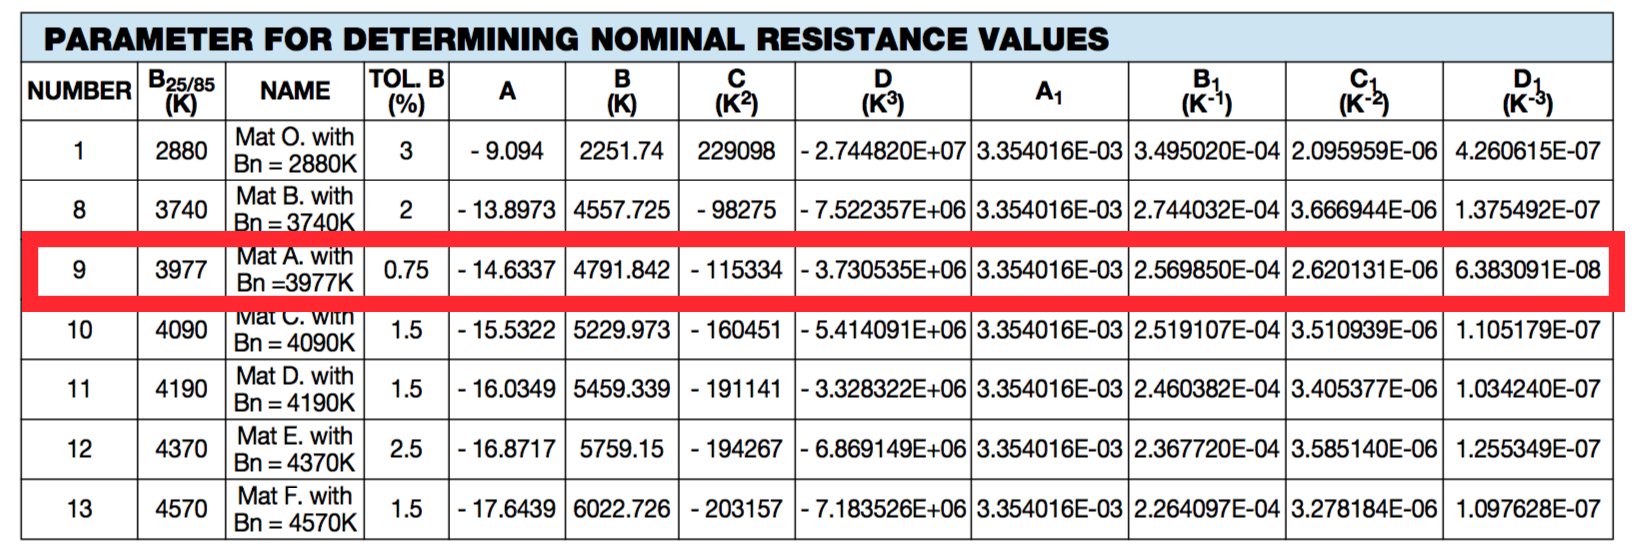
\includegraphics[width=0.6\linewidth]{images/constantes.png}
  \caption{Tableau des constantes utilisées de la datasheet du thermistor}
  \label{datasheet_constantes}
 \end{center}
\end{table}

Les Figures \ref{setup_behav_dia} et \ref{loop_behav_dia} illustrent l'implémentation du microcontrôleur. On y retrouve les deux étapes par lesquelles passe l'Arduino: le \texttt{setup} et le \texttt{loop}.\\ 


\begin{figure}[h]
 \begin{center}
  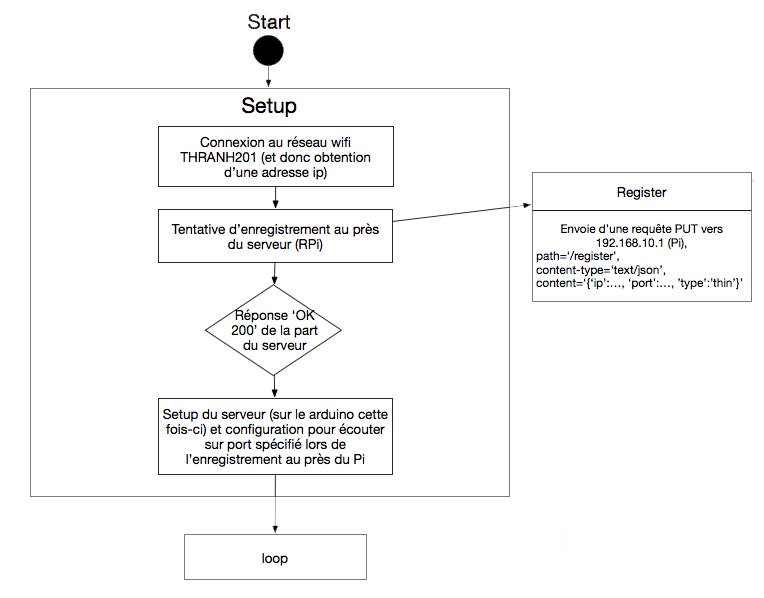
\includegraphics[width=\linewidth]{images/setup_behav_dia.png}
  \caption{Schéma des étapes d'initialisation d'un arduino}
  \label{setup_behav_dia}
 \end{center}
\end{figure}

Le \texttt{setup} se lance à la mise sous tension de l'Arduino et est effectué une seule fois. Il est donc logique d'y retrouver la fonction d'initialisation de connexion au Wi-Fi du serveur et celle d'enregistrement. La valve thermostatique est également initialisée à 0.\\

Le \texttt{loop}, quant à lui, est la boucle qui tourne tant que l'Arduino est sous-tension. Il vérifie à intervalle régulier qu'aucune requête ne lui est adressée. Dans le cas échéant, il découpe la requête et compose sa réponse en fonction de celle-ci. Si elle est bien adressée, alors il renvoie l'information demandée en respectant le protocole HTTP. Sinon, il envoie la réponse \og 400 \fg ~au serveur.\\

\begin{figure}[h]
 \begin{center}
  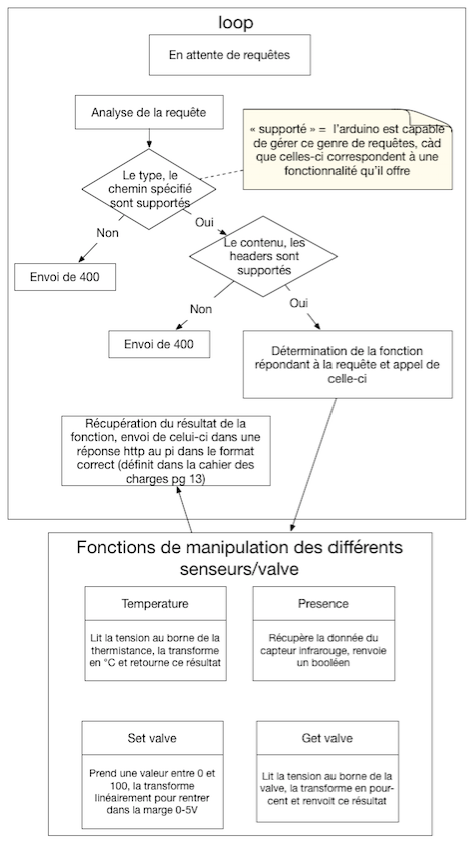
\includegraphics[width=0.63\linewidth]{images/loop_behav_dia.png}
  \caption{Schéma du comportement d'un arduino}
  \label{loop_behav_dia}
 \end{center}
\end{figure}

%--------------------------------------------------------------------------------------
%	THERMOSTAT CENTRAL
%--------------------------------------------------------------------------------------

\chapter{Thermostat central}

\section{Serveur}

Cette partie est dédiée à la description du module \texttt{ThermoServer} dont le but principal est de gérer les Arduino connectés (dès la connexion et pendant la récolte des mesures). Il a été implémenté de façon à répondre strictement à la description du protocole de communication du cahier des charges. Son fonctionnement global est synthétisé sur la Figure \ref{server_behav_dia}. L'implémentation est telle qu'il est très facile de créer et de gérer de nouveaux types de senseur (autres que ceux de type \og thin\fg ~et \og outside\fg  ~demandés dans le cahier des charges).

\begin{figure}
\centering
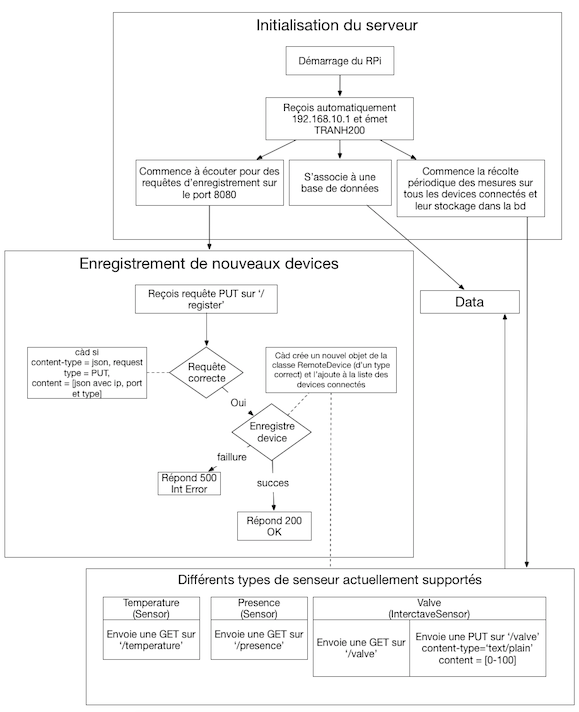
\includegraphics[width=\textwidth]{images/server_behav_dia.png}
\caption{Schéma du comportement du serveur}
\label{server_behav_dia}
\end{figure}

\subsection{Implémentation}
\begin{figure}
\makebox[\textwidth][c]{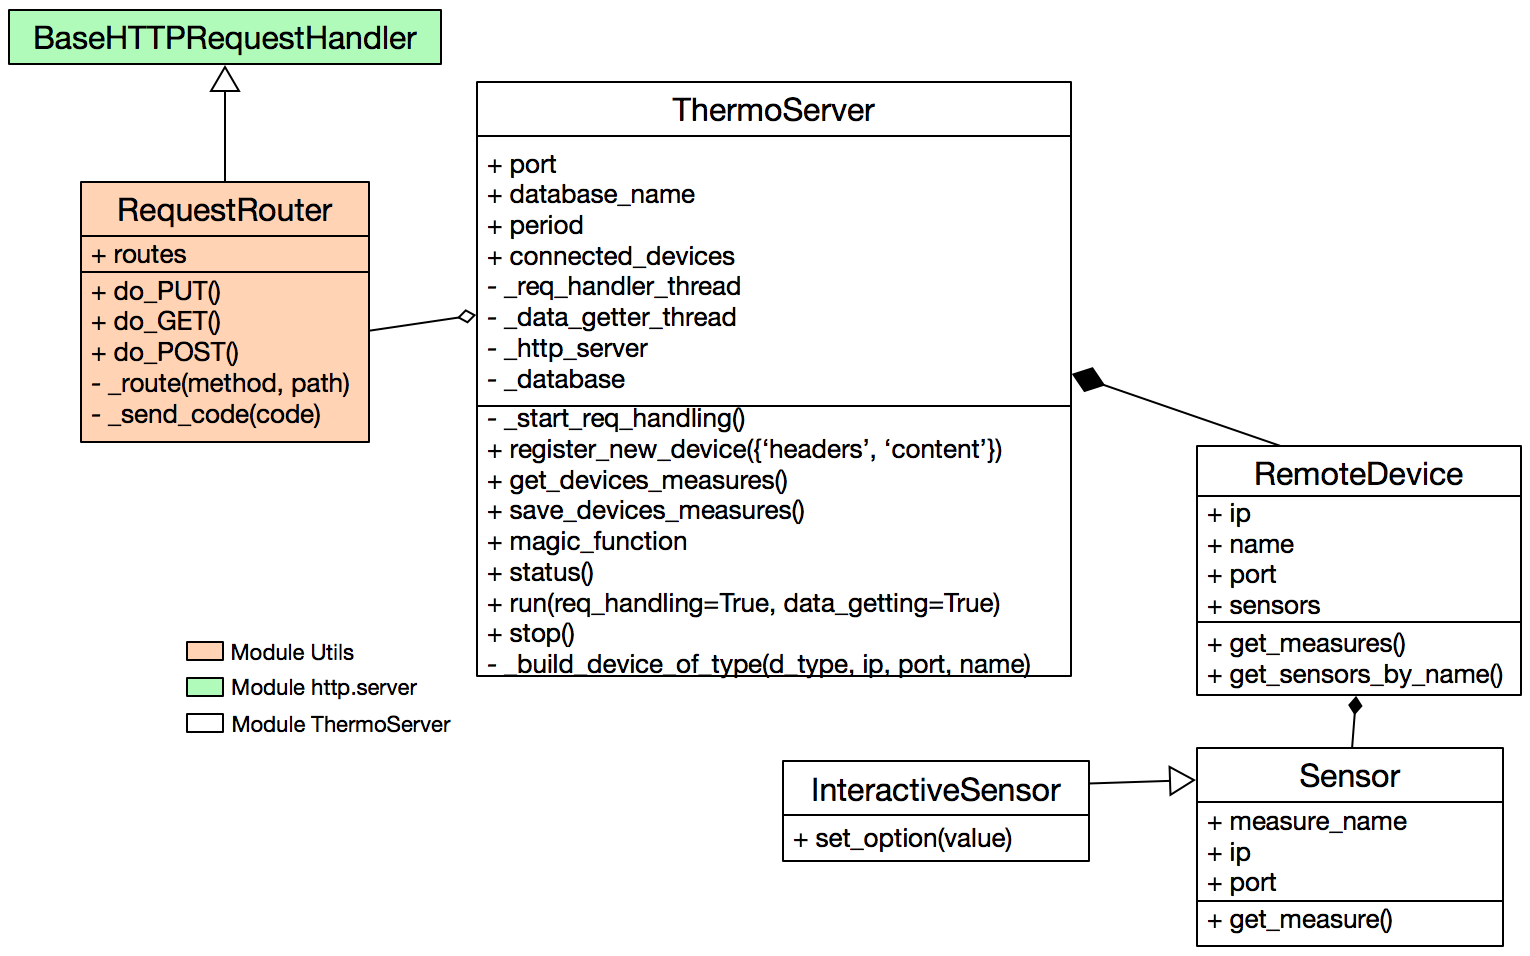
\includegraphics[width=1.15\textwidth]{images/ThermoServer_class_diagram.png}}
\caption{Diagramme de classes du module ThermoServer}
\label{ThermoServer_class_diagram}
\end{figure}

Le protocole de communication s'appuie sur un ensemble de classes qui interagissent entre elles, chacune effectuant une tâche bien précise (décrites brièvement dans le diagramme de classes présenté à la Figure \ref{ThermoServer_class_diagram}\footnote{Comme mentionné précédemment, les diagrammes de classes présentés dans ce rapport s'inspirent des règles proposés par l'UML mais ne sont pas strictement corrects du point de vue de ce langage. Leur but étant principalement documentaire, une trop grande rigueur n'a pas été jugée utile.}). Chacune d'elles sont détaillées dans les sections suivantes.

\subsubsection{\texttt{ThermoServer}}
\texttt{ThermoServer} est la classe principale de ce serveur. Son but est de s'occuper simultanément de l'enregistrement des Arduinos, de la récupération et de l'enregistrement de leurs mesures dans une base de données et de la programmation de l'horaire de contrôle des vannes thermostatiques connectées. Ces fonctions sont également réparties sur les autres classes de ce module ainsi que sur les modules \texttt{Data}, \texttt{Utils} ainsi que tous ces gerant l'aspect réactif et l'intelligence du thermostat.\\

Plus techniquement, cette classe est initialisée au démarrage du Raspberry et lance un premier thread consacré au serveur enregistrant les Arduino qui tentent de se connecter (à l'aide de la classe \texttt{RequestRouter} décrite dans la partie \ref{Utils}), et un second récoltant périodiquement les mesures renvoyées par les thermostats auxiliaires connectés et les stockant dans une base de données dédiée. Cette classe envoie également les requêtes de contrôle des vannes thermostatiques.


\subsubsection{\texttt{RemoteDevice}}

Cette classe sert d'interface de communication pour les Arduino. Une instance de celle-ci est créée à chaque connexion d'un nouveau Remote Device et permettra d'envoyer chaque requête pour récupérer chacune de ses mesures et pour contrôler ce qui est modulable (les vannes par exemple).\\

De façon plus technique, cette classe est décrite par une adresse IP et un port permettant la communication avec l'Arduino, par un nom identifiant ces mesures et une liste de senseurs qui sont branchés sur ce thermostat auxiliaires. Cette liste permet de créer tout type de Remote Device, composé de plusieurs senseurs, tels qu'une thermistance, un capteur de présence ou même d'humidité, ou tout autre type de mesures imaginables et compatibles avec le circuit et le code de l'Arduino.\\

Grâce à cette implémentation modulaire des Remote Devices, il est possible de créer des objets connectés de tout type et pas seulement de type "thin" ou "outside" comme décrit dans le cahier des charges. L’évolution et l'expansion du projet est rendue beaucoup plus facile sans pour autant compliquer l'implémentation de ce qui est demandé.\\

\subsubsection{\texttt{Sensor}}

Une instance de cette classe permet simplement de récupérer la mesure du senseur correspondant. Par exemple, si l'on imagine un Arduino sur lequel est connecté une thermistance et configuré pour renvoyer la température ambiante en réponse à une requête de type \texttt{GET} sur le chemin \texttt{temperature}, cet objet de type \texttt{Sensor} permettra d'envoyer cette requête et de récupérer la température. \\

Dans le cadre du protocole de communication implémenté ici, un objet de type \texttt{Sensor} est créé pour chaque senseur physique branché et configuré à chaque Remote Device connecté au serveur.

\subsubsection{\texttt{InteractiveSensor}}

Cette classe hérite de la classe \texttt{Sensor} décrite ci-dessus en ajoutant la possibilité d'envoyer une requête de type \texttt{PUT} à un senseur pour le contrôler à distance. Typiquement, cette classe permet de récupérer ET de modifier l'état d'ouverture d'une vanne thermostatique. Dans le cadre du projet, elle est typiquement associée à la valve.


\subsubsection{\texttt{LocalSensor}}

Cette classe possède le même comportement qu'une \texttt{InteractiveSensor} dans le sens ou une de ses instance elle représente une mesure utilisée par un Remote Device. La différence ici c'est que cette mesure est stockée sur le serveur et prend la forme d'une variable.\\


%%%%%%%%%%%%%%%%%%%%%%%%%%%%%%%%%%%%%%%%%%%%%%%%%%%%
%  DATA
%%%%%%%%%%%%%%%%%%%%%%%%%%%%%%%%%%%%%%%%%%%%%%%%%%%%
\newpage
\section{Gestion des données}

\subsection{Introduction}

\paragraph*{}
  Afin d'implémenter une analyse intelligente des habitudes de l'utilisateur, un système de stockage de données est nécessaire. Deux options sont envisageables. Soit une structure sous forme de fichier, soit une autre utilisant les bases de données. Des recherches ont été menées pour déterminer quel système serait le plus adéquat. Il en est ressorti que les bases de données correspondent mieux à la problématique. En effet, celles-ci sont plus rapides, plus simples à manipuler et s'adaptent facilement à différentes tailles de jeux de données. De plus, en Python, de nombreuses bibliothèques les concernant existent, et certains types de bases de données, comme par exemple SQLite, y sont intégrés par défaut. Les raisons citées précédemment ont dès lors mené à une décision en faveur des bases de données.


% Termes subjectifs: "simple", "plus adéquat"?? (Gros chipotage)

\subsection{Choix du gestionnaire base de données}
\paragraph*{}
  Il existe différents SGBD\footnote{Système de Gestion de Base de Données}, chacun ayant ses avantages et inconvénients. Une analyse comparative des plus populaires a été réalisée et SQLite a été choisi. La Table \ref{tableau db} justifie cette décision. 

\begin{table}[h]
   \centering
   \begin{tabularx}{\linewidth}{|c||X|X|X|}
      \hline
       Caractéristiques & \centering{SQLite} & \centering MySQL & \centering PostgreSQL \tabularnewline
      \hline
      Installation & Module SQLite déjà implémenté dans Python.\cite{table1} & Installation d'un serveur MySQL nécessaire.\cite{table2} & Installation de PostgreSQL nécessaire.\cite{table3}\tabularnewline
      \hline
      Types de données supportés & NULL, INTEGER, REAL, TEXT, BLOB.\cite{table4} & Complet, accepte également des entrées de type \og Date \fg.\cite{table5} & Complet, accepte également des entrées de type \og Date \fg.\cite{table6} \tabularnewline
      \hline
    Stockage de la base de donnée & La base de donnée est condensée en un seul \og fichier \fg ~stocké directement dans la mémoire (Du Raspberry dans ce cas).\cite{table7}  & La base de donnée est stockée sur un serveur au quel doivent se connecter les utilisateurs.\cite{table8}& La base de donnée est stockée sur un serveur au quel doivent se connecter les utilisateurs.\cite{table9}\\    
		\hline
	\end{tabularx}
\caption{\label{tableau db} Tableau comparatif des différents SGBD étudiées}
\end{table}

\subsection{Implémentation} % TODO: j'aipas encore finit, il faut encore changer les digagramme et mettre en page. Il y a juste les idées qui sont la..


\paragraph*{}
L'implémentation du module \texttt{Data} consiste en trois classes, \texttt{ThermoDB}, \texttt{QueryHandler} et 
\newline
\texttt{ThermoQueryHandler} ayant chacune un rôle distinct. Elle est construite selon une structure de base de données formée de deux tables \emph{measure} et \emph{device} jointes par une relation many-to-one (voir Figure \ref{Data_class_diagram}) % TODO: référence.

\begin{figure}
\centering
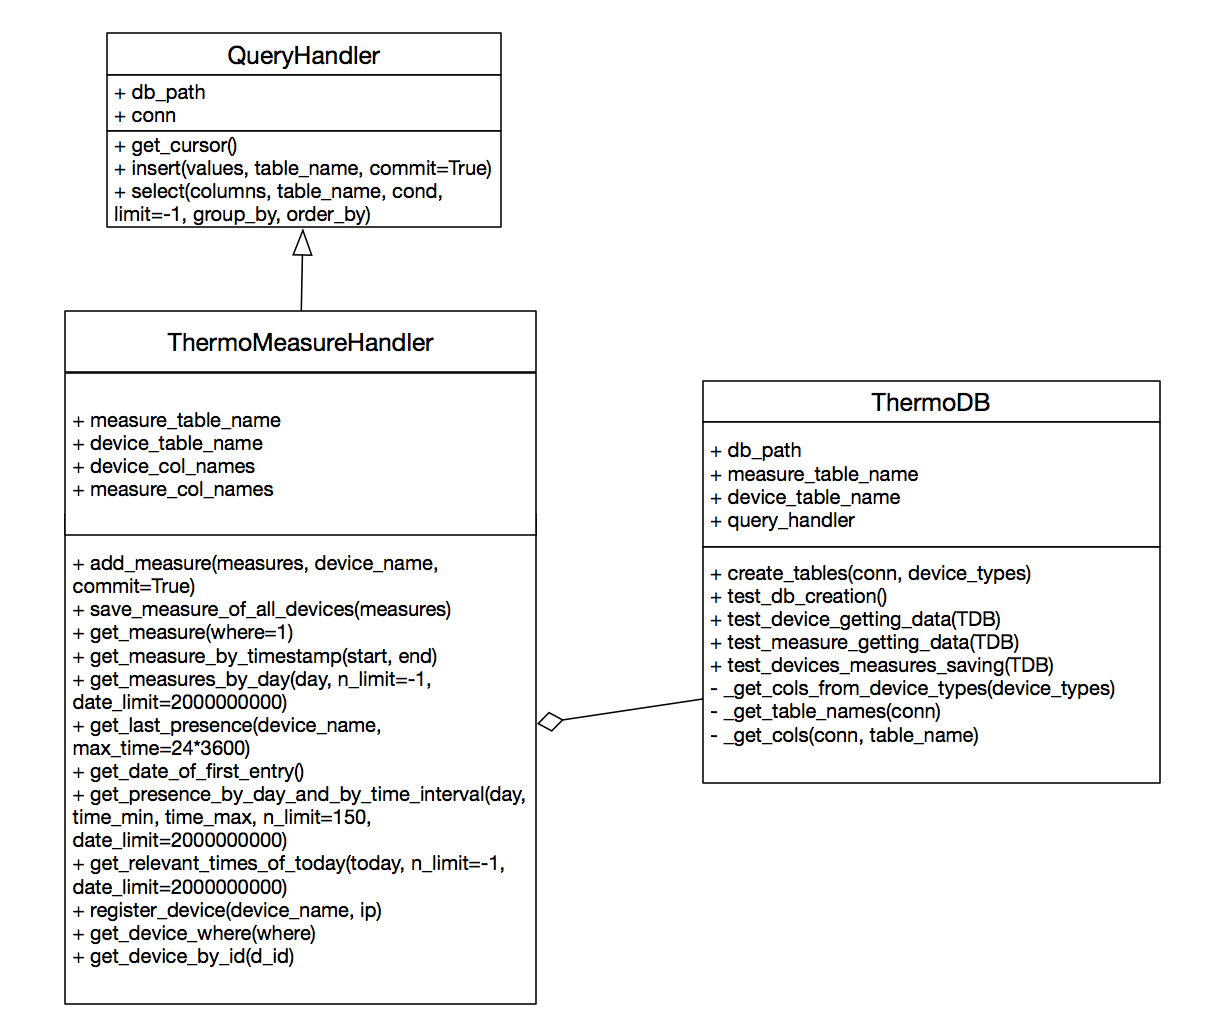
\includegraphics[width=0.5\textwidth]{images/Data_class_diagram.png} % TODO: new diagram
\caption{Diagramme de classe du module \texttt{Data}}
\label{Data_class_diagram}
\end{figure}

\subsubsection{\texttt{ThermoDB}}

Cette classe s'occupe de la création (processus lancé à l'initialisation du serveur) ou de la récupération (et de la vérification de la validité) d'une base de donnée existante. Ce qui peut être utile en cas de redémarrage du serveur.


\subsubsection{\texttt{QueryHandler}}

Il s'agit d'une classe pseudo-abstraite\footnote{Dans le sens où elle a été conçue pour être héritée} définissant les fonctions de récupération et d'enregistrement de données génériques. Les définir permet de centraliser l'accès à la base de données et les éventuelles erreurs qui pourraient en découler. Cela permet de faciliter le débogage et les tests. %Debogage est tres moche mais c'est le mot officiel (televerser...)

\subsubsection{\texttt{ThermoQueryHandler}}
Cette classe hérite de la précédente et définit des méthodes spécifiques à la manipulation des données relatives au thermostat. 


\iffalse
%mis en commentaire
\begin{description}
\item[ThermoDB]: s'occupe de la création de la base de donnée (processus lancé à l'initialisation du serveur) ou de la récupération (et de la vérification de la validité) d'une base de donnée existante (utile en cas de redémarrage du serveur). 
\end{description}

\begin{description}
\item[QueryHandler]: il s'agit d'une classe pseudo-abstraite (dans le sens ou elle a été concue pour être héritée) définissant les fonction de récupération et d'enregistrement de donnée générique. Définir ces fonction permet de centraliser l'accès à la base de donnée et les éventuelles erreur qui pourraient en découler à un seul endroit. Cela permet de faciliter le débugage et les tests.
\end{description}

\begin{description}
\item[ThermoQueryHandler]: cette classe hérite de la précédente et définit des méthodes spécifiques à la manipulation de données relatives au thermostat. 

\end{description}

\subsection{Utilisation du module par le thermostat}
Cette partie décrit brièvement les étapes de fonctionnement du module data lorsqu'il est utilisé par le thermostat, de l'initialisation à la manipulation de données. % TODO: référence à une diagramme d'état? \\

L'une des étape d'initialisation du thermostat central est l'initialisation de la base de donnée. Pour cela, une instance de la classe \texttt{ThermoDB} est créé. Elle s'occupe de créé une nouvelle base de donnée correctement structurée (ou utilise une base de donnée existante et valide si possible). Les colones de la table measure sont déterminées par les types de remote device supporté par le serveur.%TODO: parler de ces type dans l'implémentation du serveur plus haut!!!!
Une fois la base de donnée prête, un objet de type ThermoQueryHandler est initialisé et associé à l'instance de ThermoDB. Il permettra d'accéder aux données..

La structure adoptée pour l'instant crée une base de données et, à chaque fois qu'un Remote Device se connecte au serveur, une table portant son nom est générée comme le montre la Figure \ref{current_structure}. Le détail des classes est schématisé à la Figure \ref{Data_class_diagram} et développé dans les paragraphes suivants.
   
\begin{figure}
\centering
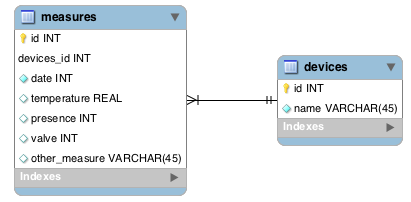
\includegraphics[width=0.75\textwidth]{images/better_structure.png}
\caption{Schéma de la structure plus adaptée envisagée}
\label{Better_structure}
\end{figure}

\begin{figure}
\centering
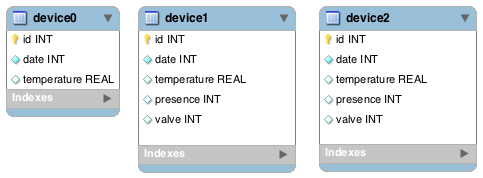
\includegraphics[width=0.9\textwidth]{images/current_structure.png}
\caption{Schéma de la structure présentement implémentée de la base de donnée}
\label{current_structure}
\end{figure}

\subsubsection{Classe \texttt{Database} }
\paragraph*{}
   La classe \texttt{Database} est l'intermédiaire entre le serveur et la base de données. Elle permet, entre autres, de créer une base de données, de s'y connecter et d'y créer des tables. Elle a été conçue de telle sorte à ne pas créer d'instabilité. En effet si le serveur vient à redémarrer, une instance identique à celle en cours précédemment est créée afin que le code continue à s'exécuter de la manière souhaitée.
    
\subsubsection{Classe \texttt{Table}}
\paragraph*{}
	Quant à elle, la classe \texttt{Table} permet d'effectuer des manipulations sur une table, comme par exemple ajouter des entrées ou en supprimer. Elle a principalement été conçue en généralisant la syntaxe du module \texttt{sqlite3} de façon à créer des méthodes d'un plus haut niveau d'abstraction et élégantes d'utilisation.
    
\subsection{Regard critique sur l'implémentation de la base de données}
\paragraph*{}
	L'implémentation actuelle du module \texttt{Data} n'est pas optimale. Cette manière de faire a été décidée tôt dans la conception du serveur. Elle a mené à de longues discussions et semblait être une bonne solution dans la mesure où elle correspondait à la structure globale du code qui consiste une indépendance des différents Remote Devices afin de rendre ce dernier plus flexible. Par la suite, il s'est avéré que ce n'est pas une bonne structure à adopter. En effet, ce n'est pas une façon propre de faire car cela va à l'encontre des règles de bonnes pratiques. Lorsqu'une base de données est utilisée, afin d'optimiser les performances, une seule et unique table est utilisée. De plus, si il y a des problèmes de connexion et que le serveur oublie l'existence des Remote Devices, à chaque fois que ceux-ci se reconnecteront des nouvelles tables seront créées, potentiellement en très grands nombres.
    
\paragraph*{}
	Ces raisons motivent le fait qu'une nouvelle structure soit implémentée dès que possible. Celle-ci s'articule comme l'indique la figure \ref{Better_structure}. Une seule grande table contiendra toutes les données de tous les Remote Device, peu importe leur type, et aura en plus un identifiant qui fera le lien avec le Remote Device d'où proviennent les données correspondantes grâce à une table de jointure. De cette manière, le système gagne en flexibilité car il est possible d'ajouter n'importe quel type de capteur\footnote{Dans une perspective de développement ultérieur du projet, par exemple ajouter des capteurs d'humidité,...} sur les Remote Devices, ce qui est le résultat recherché.
    
    %to do: j'aurai mis les graphiques ici vu que c'est dans ce paragraphe que tu y fais référence
\fi


%%%%%%%%%%%%%%%%%%%%%%%%%%%%%%%%%%%%%%%%%%%%%%%%%%%%
%  Régulateur PID
%%%%%%%%%%%%%%%%%%%%%%%%%%%%%%%%%%%%%%%%%%%%%%%%%%%%

%\newpage

\section{Régulation en boucle fermée}

\subsection{Le choix du régulateur}

Un des objectifs du régulateur est d'atteindre une valeur consigne, qui est dans ce cas-ci une température désirée. Un autre de ses objectifs est d'atteindre cette objectif avec stabilité (Sans oscillations autour de cette valeur) et ceci le plus rapidement possible. Il n'est en effet pas intéressant d'avoir un régulateur qui permette à la température de constamment varier\footnote{Ce qui consomme de l'énergie d'éteindre et rallumer le système de chauffage. Dans le cas d'un thermostat, on parle du phénomène de pompage} ou qui n'atteint pas la valeur consigne d'une manière optimale. 3 types de régulateurs ont été comparés : le régulateur "On/Off", le régulateur "PID"\footnote{PID pour "Proportional Integral Derivative"} et le régulateur "LQR"\footnote{LQR pour "Linear-Quadratic Regulator"}\footnote{Bien qu'il existe d'autres régulateurs, ce dernier n'étany pas le sujet central de ce travail il ne semble pas intéressant d'en comparer un plus grand nombre. A ce titre, peuvent être cités comme régulateur: "Fuzzy control", "Process reaction method", "Fuzzy PID control", "Adaptive control" ou encore "Sliding Mode Control"} (Voir Tableau \ref{regulateur}).

\begin{table}[h]
   \centering
   \begin{tabularx}{\linewidth}{|c|X|X|X|}
      \hline
       Caractéristiques & \centering{ Régulateur On/Off} & \centering Régulateur PID & \centering Régulateur LQR \tabularnewline
      \hline
      Performance &\centering{ - } & \centering ++ &\centering +++\tabularnewline
      \hline
      Stabilité &\centering{ - } & \centering ++ &\centering ++\tabularnewline
      \hline
      Facilité d'implémentation &\centering{ +++ } & \centering ++ &\centering -\tabularnewline
      \hline

	\end{tabularx}
\caption{\label{regulateur} Tableau comparatif des différents régulateurs}
\end{table}

Il clairement que le régulateur PID est le plus adéquat. En effet, il a été étudié que cette méthode est également quantitativement plus intéressante\footnote{Facilité d'implémentation : Notamment au niveau de la paramétrisation du jeu de constantes utilisées}\footnote{A nouveau, l'analyse de graphique de performance de performance n'étant pas le sujet principal de ce travail, le lecteur est renvoyé vers la bibliographie pour plus de détails sur ces études}.

%TO DO je dois encore rajotuer ds la biblio : "Comparison Performance Between PID and LQR Controllers"
%TO DO entourer la colonne du régulateur PID pour montrer notre choix
%TO DO; il faut rajouter le schéma d'un régulateur en boucle fermée?? C'est nécessaire?

\subsection{Régulateur PID}

\subsubsection{Relation mathématique}

Le régulateur PID peut être résumé par la relation:

\begin{equation}
\label{equation_pid}
	u(t) = K_p e(t) + K_i \int_0^t{e(\tau)d\tau} + K_d\frac{d}{dt}e(t)
\end{equation}

%On rajoute la forme laplacienne?? J'suis pas sur d'avoir compris à quoi elle servait ds notre cas vu qu'on fait pas de modélisation ac des équa diff
%On va utiliser le D aussi? pcq des études montrent que c'est pas nécessaire

où t représente le temps, e(t) représente l'erreur\footnote{Ici, l'erreur représente la différence entre la température demandée (valeur consigne) et la température mesurée} et u(t) sera la sortie de notre régulateur qui dépendra des 3 constantes $K_p$,$K_i$ et $K_d$, respectivement constantes de la proportionnelle, de l'intégrale et de la dérivée. Celles-ci doivent être déterminées et ce protocole sera explicité dans les sections qui suivent.

\subsubsection{Ajustement des constantes}

Deux voies sont possibles pour l'ajustement des constantes. La première consiste en l'utilisation de calculs d'équations de chaleur, la deuxième permettant plutôt de les obtenir expérimentalement. Elles s'obtiennent en les déterminant une à une successivement. En effet, il faut commencer par utiliser un régulateur P proportionnel et de régler la constante du gain proportionnel en fonction du résultat attendu. Une fois fixé, on utilise un régulateur PI pour fixer la constante du gain intégral et enfin un régulateur PID pour fixer la troisième constante. L'objectif final étant d'obtenir une courbe comme celle de la figure \ref{PID}, sans aucune oscillation.\\

Il est cependant beaucoup plus judicieux que ces constantes se déterminent automatiquement et qu'elles s'adaptent de manière pro-active. De plus, il faut que ce système soit le plus \textit{user-friendly} possible afin que tout le monde puisse profiter du thermostat sans aucune connaissance en physique ou informatique.\\

Un algorithme d'initialisation automatique et optimisé des constantes a été développé. Ce dernier permet comme explicité précédemment d'obtenir, après plusieurs jours d'utilisations, une approche assez fidèle des constantes \og réelles \fg. Les explications associées sont présentes dans la section qui traite de la partie \ref{opti_pid}.

\subsubsection{Implémentation du PID dans le serveur central}
\label{pid_section}

Deux classes principales sont implémentées : \texttt{PID} et \texttt{PIDHandler}. \\

La première possédant les méthodes nécessaires au calcul de l'erreur (Température effective - Température cible), de la dérivée de l'erreur et de l'intégrale de l'erreur. Ces trois valeurs sont les valeurs présentes dans l'équation \ref{equation_pid}. Deux autres méthodes sont également présentes : \texttt{update} et \texttt{set\_constants}. La première permet d'actualiser les attributs de la classe PID concernant la température (visée/effective), la date ou l'ouverture de la valve tandis que la deuxième s'occupe exclusivement de gérer les constantes du régulateur : $K_p$, $K_i$, $K_d$.\\

Le rôle de la deuxième sera détaillé à la section \ref{opti_pid} du chapitre \ref{intelligence}.\\

\section{Module \texttt{Utils}} % TODO: mettre à jour
\label{Utils}
Ce module contient trois classes principales : \texttt{RepeatingTimer}, \texttt{RequestRouter} et
\newline
\texttt{TimeOperator}. \\

Il a pour but de contenir des classes ou plus généralement des outils qui sont complètement indépendants du projet (mais utiles à celui-ci) et qui pourraient donc être facilement utilisables pour un quelconque autre projet. Outre le fait que la séparation des classes génériques leur permet d'être réutilisées dans d'autre projet, se pliant ainsi aux règles de bonnes pratiques, la construction d'un module séparé contenant ces classes permet d'alléger les autres modules et de les rendre plus compréhensible.\\


Ces deux classes sont donc construites de façon générique et accomplissent des taches élémentaires.


\subsection{\texttt{RepeatingTimer}}

\begin{figure}[h]
\centering
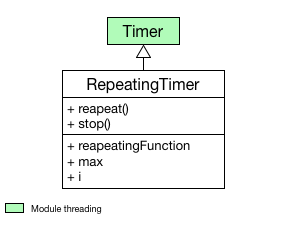
\includegraphics[width=0.5\textwidth]{images/RepeatingTimer_class_diagram.png}
\caption{Diagramme de classe pour \texttt{RepeatingTimer}}
\end{figure}

La seule fonction de cette classe (héritant de la classe \texttt{Timer} du module \texttt{threading} de python) est d'appeler une fonction spécifiée à intervalle régulier.
Elle est utile, dans ce projet, à la collecte régulière des mesures du serveur sur les remote devices connectés.\\

\subsection{\texttt{RequestRouter}}

\begin{figure}[h]
\centering
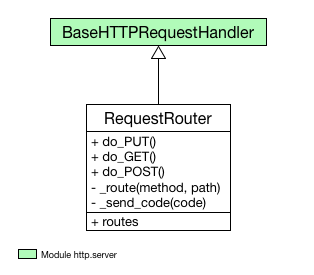
\includegraphics[width=0.5\textwidth]{images/RequestRouter_class_diagram.png}
\caption{Diagramme de classe pour \texttt{RequestRouter}}
\end{figure}

Cette classe, héritant de \texttt{BaseHTTPRequestHandler} fournie dans le module \texttt{http.server} de python 3, a pour but d'écouter sur un port spécifié pour d'éventuelles requêtes et de les "router" vers un callback spécifié en fonction de la méthode http et du chemin de la requête.\\

Elle est totalement générique puisque n'importe quelle requête peut déclencher n'importe quelle fonction (pour peu qu'elle soit configurée correctement) et peut-être utilisée dans n'importe quel cas nécessitant un serveur.\\

Dans le cadre spécifique de ce projet, cette classe est utile à la réception et au traitement des requêtes d'enregistrement des remote devices.

\subsection{\texttt{TimeOperator}}

Cette classe possèdes des méthodes statiques\footnote{Cette classe ne présentait pas d'intérêt à devoir être instanciée.} ayant pour but d'effectuer les opérations temporelles nécessaires aux modules intelligents présentés à la section \ref{intelligence}. Elle est détaillée à la figure \ref{timeoperator}.

\begin{figure}[h]
\centering
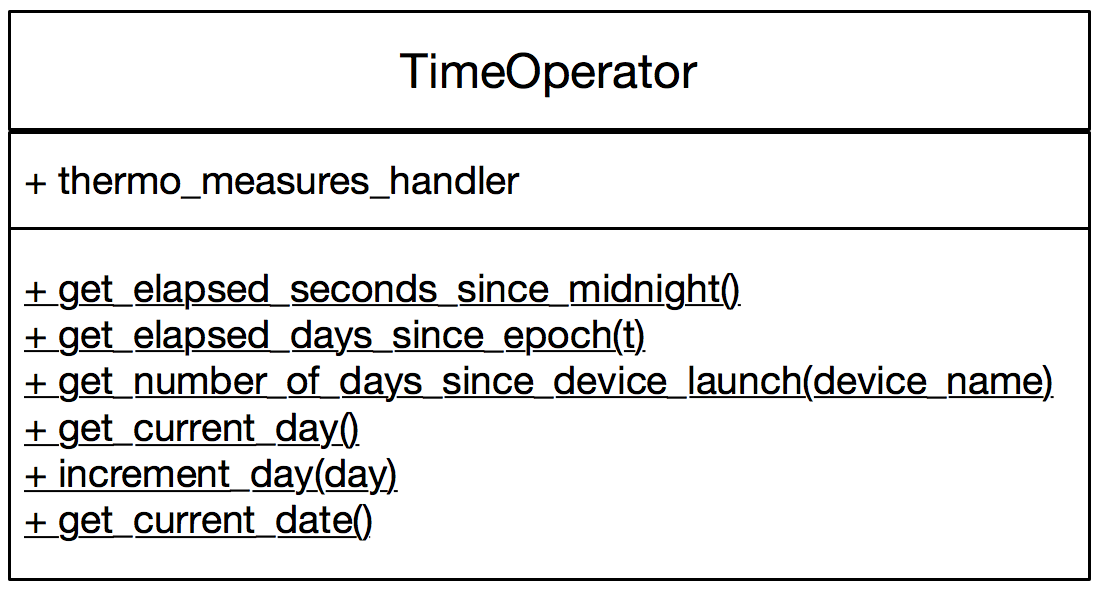
\includegraphics[width=0.5\textwidth]{images/TimeOperator_class_diagram.png}
\caption{Diagramme de classe pour \texttt{TimeOperator}}
\label{timeoperator}
\end{figure}

\section{Débogage}

Un système de logging est implémenté dans tous les modules pour garder une trace de chaque éventuelle erreur, dysfonctionnement ou anomalie lors de l'exécution du serveur. Le dépannage est alors simplifié lors d'une utilisation réelle et le débogage est plus rapide lors du développement dès lors que l'origine des erreurs est plus facilement identifiable. Il est ainsi possible dès le lancement du serveur d'indiquer quels types (niveau de gravité) de messages doivent être affichés et/ou stockés dans un fichier journal.


\chapter{Intelligence du code}
\label{intelligence}

\section{Introduction}
Cette partie concerne les modules utilisés par le serveur afin de rendre le thermostat prédictif. Elle présente trois objectifs principaux qui ont pour but de rendre le système autonome. Un premier module calcule des probabilités en se basant sur la base de données et fournit des prédictions de présence, un second optimise les constantes du contrôleur PID afin qu'il s'adapte à n'importe quelle pièce et finalement, un dernier y fait appel pour évaluer le temps nécessaire pour atteindre la température désirée. \\

\section{Critères d'intelligence}
\label{critere_intelligence}

L'objectif principal d'un thermostat intelligent est de minimiser les dépenses énergétiques liées à la régulation thermique tout en assurant à ses utilisateurs un confort au minimum égal à celui offert par un dispositif traditionnel. \\

Ces deux aspects sont étudiés ici. Tout d'abord il est nécessaire de définir les notions de consommation énergétique et de confort thermique\footnote{Ces définitions ont été définies sur base d'articles traitant de ce sujet.}. La première a été standardisée \cite{confort_thermique} et dépend de nombreux paramètres (humidité, température, aération, ...). Cependant, dans le cadre de ce projet et par souci de simplification, seule la température intérieure est étudiée. Il a donc été supposé que le confort maximal est atteint lorsque la différence entre la température actuelle et la température désirée par l'utilisateur est minimale\footnote{Cet objectif sera atteint au moyen de la régulation PID}.\\

Concernant la consommation énergétique, il a été considéré qu'elle serait minimisée à condition de raccourcir un maximum les périodes de chauffe\footnote{Ceci au moyen des prédictions de présence.} ainsi qu'en réduisant l'oscillation de la température désirée autour de celle effective.\\

\iffalse

\section{Formules}
En démarrant de l'équation \ref{equation_pid}, et en posant a, b et c de la manière suivante :
\begin{equation}
\left\{
\begin{aligned}
& a_{i} = \int_{t_{0}}^{t_{i}}e(\tau)d\tau\\
& b_{i} = \frac{de(t_{i})}{dt}\\
& c_{i} = (T_{T}(t_{i})-T(t_{0}))\\
%& b_{i} = \int_{t_{0}}^{t_{i}}\int_{t_{0}}^{t}e(\tau)d\tau dt\\
%& c_{i} = (e(t_{i})-e(t_{0}))
\end{aligned} \right.
\end{equation}
On arrive au système d'équation suivant :

\begin{equation}
\sum_{i=0}^{n}(T(t_{t0}) + K_{p}e(t_{i}) + K_{i}a_{i} + K_{d}b_{i} - T_{T}(t_{i}))^{2}\\
\end{equation}

Et lorsque l'équation est dérivée en fonction de ses variables qu'on égalise à zéro on a:
\begin{equation}
\left\{
\begin{aligned}
& K_{p}\sum_{i=0}^{n}(e(t_{i}))^{2} + K_{i}\sum_{i=0}^{n}a_{i}e(t_{i}) + K_{d}\sum_{i=0}^{n}b_{i}e(t_{i}) = \sum_{i=0}^{n} e(t_{i})c_{i}\\
& K_{p}\sum_{i=0}^{n}e(t_{i})a_{i} + K_{i}\sum_{i=0}^{n}(a_{i})^{2} + K_{d}\sum_{i=0}^{n}b_{i}a_{i} = \sum_{i=0}^{n} a_{i}c_{i}\\
& K_{p}\sum_{i=0}^{n}e(t_{i})b_{i} + K_{i}\sum_{i=0}^{n}a_{i}b_{i} + K_{d}\sum_{i=0}^{n}(b_{i})^{2} = \sum_{i=0}^{n} b_{i}c_{i}\\
\end{aligned} \right.
\end{equation}

\fi

\iffalse 
%Pour mettre tout en commentaire

\begin{equation}
\left\{
\begin{aligned}
& K_{p}\sum_{i=0}^{n} a_{i}^{2} + K_{i}\sum_{i=0}^{n}(a_{i}b_{i}) + K_{d}\sum_{i=0}^{n}(a_{i}c_{i}) = \sum_{i=0}^{n} a_{i} (T_{T}(t_{i})- T(t_{0}))\\
& K_{p}\sum_{i=0}^{n} (a_{i}b_{i}) + K_{i}\sum_{i=0}^{n} b_{i}^{2} + K_{d}\sum_{i=0}^{n} (b_{i}c_{i}) = \sum_{i=0}^{n} b_{i} (T_{T}(t_{i})- T(t_{0}))\\
& K_{p}\sum_{i=0}^{n} (a_{i}c_{i}) + K_{i}\sum_{i=0}^{n} (b_{i}c_{i}) + K_{d}\sum_{i=0}^{n} c_{i}^{2} = \sum_{i=0}^{n} c_{i} (T_{T}(t_{i})- T(t_{0})))
\end{aligned} \right.
\end{equation}

\begin{equation}
\left\{
\begin{aligned}
& K_{p}\sum_{i=0}^{n} (\int_{t_{0}}^{t_{i}}e(t)dt)^{2} + K_{i} \sum_{i=0}^{n} \int_{t_{0}}^{t_{i}}\int_{t_{0}}^{t}e(\tau)d\tau dt \int_{t_{0}}^{t_{i}}e(t)dt + K_{d} \sum_{i=0}^{n} (e(t_{i})-e(t_{0})) \int_{t_{0}}^{t_{i}}e(t)dt = \sum_{i=0}^{n} \int_{t_{0}}^{t_{i}}e(t)dt (T_{T}(t_{i})- T_{T}(t_{0}))\\
& K_{p}\sum_{i=0}^{n} \int_{t_{0}}^{t_{i}}e(t)dt + \int_{t_{0}}^{t_{i}}\int_{t_{0}}^{t}e(\tau)d\tau dt + K_{i} \sum_{i=0}^{n} (\int_{t_{0}}^{t_{i}}\int_{t_{0}}^{t}e(\tau)d\tau dt)^{2} + K_{d} \sum_{i=0}^{n} (e(t_{i})-e(t_{0}))\int_{t_{0}}^{t_{i}}\int_{t_{0}}^{t}e(\tau)d\tau dt = \sum_{i=0}^{n} \int_{t_{0}}^{t_{i}}\int_{t_{0}}^{t}e(\tau)d\tau dt (T_{T}(t_{i})- T_{T}(t_{0})) \\
&  
\end{aligned} \right.
\end{equation}


\fi

\section{Prédiction de présence}
\label{Prediction_presence}

\subsection{Introduction}
%Pour que le système soit le plus pertinent et efficace possible, il doit être en mesure de calculer la probabilité qu'il y ait une présence en tout temps. Dans cette optique, 

%La dénomination d'un thermostat intelligent ne peut prendre tout son sens que lorsque le serveur central est capable, à partir des données récoltées, de prédire des comportements chez son utilisateur. Notre modélisation mathématique du problème se base sur l'interpolation polynomiale. En somme, en analysant pour chaque jour de la semaine, si l'utilisateur est présent ou pas, il nous sera possible de déterminer ses habitudes de vies.\\ 

%Ainsi, l'utilisateur qui quitterait son appartement chaque lundi à 7h et rentrerait chez lui à 17h aurait une courbe de probabilité supérieur à 0,5 entre 17h et 7h. Le serveur central pourra donc ordonner la vanne de s'ouvrir à un temps t précédant sa probable présence pour chauffer la pièce et afin que l'utilisateur soit accueilli sous les meilleures conditions de confort possible.\\

Pour que le système soit prédictif, il doit être capable d'estimer les chances de présence de l'utilisateur dans une pièce à un instant donné. Afin de rationaliser cette démarche, il est utile d'aborder l'analyse prédictive, celle ci usant entre autre de probabilités et de statistiques. Le code présenté dans cette section a pour but de générer et manipuler un modèle mathématique consistant en une fonction associée à une probabilité en tout temps. La méthode utilisée sera : \og l'interpolation polynomiale \fg \cite{interpolation_polynomiale}. Cela consiste en la représentation de la fonction par un polynôme dont les constantes sont calculées par analyse statistique des mesures récoltées et stockées dans la base de données. Ces dernières seront comparées au valeurs effectivement observées.\\

D'autres méthodes comme les séries chronologiques ou même les séries de Fourrier auraient pu être utilisées, mais l'utilisation d'un polynôme semblait être plus simple et suffisant. L'implémentation du calcul automatique des coefficients de Fourrier et leur actualisation aurait pu se révélée bien plus complexe et fastidieux.

%to do: expliquer d'autres modèles? Ex: série chronologiques

\subsection{Modélisation mathématique}
\label{proba_math}
Le but de ce calcul est d'obtenir la fonction de probabilité introduite précédemment. Sa structure sera polynomiale afin de calculer ses constantes par interpolation.

\begin{equation}
\label{probability_function}
p : \mathbb{R}^{+} \rightarrow [0;1] : t \mapsto At^{5}+Bt^{4}+Ct^{3}+Dt^{2}+Et+F
\end{equation}

Comme présenté dans l'équation \ref{probability_function}, c'est une fonction de degré 5. Ce choix arbitraire a pour but de concilier une interpolation\footnote{Plus le degré du polynôme est élevé, meilleure sera l'interpolation.} de qualité suffisante avec un temps de calcul acceptable\footnote{Si le polynôme est de degré n, la matrice du système d'équation à résoudre sera d'ordre n+1.}.\\

La méthode appliquée pour calculer les constantes optimales consiste en une minimisation du carré\footnote{Afin de ne pas avoir d'annulation de valeurs} de la somme des différences entre le polynôme et la probabilité à approcher en tout temps. Si la probabilité mesurée est exprimée comme :

\begin{equation}
E(t_{i}) = \frac{n(t_{i})}{N(t_{i})}
\end{equation}
Avec $n(t_{i})$ correspondant au nombre de présence et $N(t_{i})$ au nombre total de prises de mesures à l'instant $t_{i}$\footnote{$t_{i}$ sera considéré par la suite comme un intervalle, ce qui justifie cette modélisation.}. Cette grandeur est toujours comprise entre 0 et 1, ceci justifiant l'utilisation de l'aspect probabiliste du problème.\\

Dès lors, l'expression à minimiser prend cette forme : 

\begin{equation}
\sum_{i=0}^{n} (p(t_{i}) - E(t_{i}))^2
\end{equation}

En égalant le gradient de cette expression au vecteur nul, et en posant $k_{j} = \sum_{i=0}^{n} t_{i}^{j}$ et $l_{s}=\sum_{i=0}^{n} E(t_{i})t_{i}^{s}$, le système à résoudre est obtenu : 

\begin{equation}
\left\{
\begin{aligned}
\label{proba_system}
&Ak_{10}+Bk_{9}+Ck_{8}+Dk_{7}+Ek_{6}+Fk_{5} = l_{5}\\
&Ak_{9}+Bk_{8}+Ck_{7}+Dk_{6}+Ek_{5}+Fk_{4} = l_{4}\\
&Ak_{8}+Bk_{7}+Ck_{6}+Dk_{5}+Ek_{4}+Fk_{3} = l_{3}\\
&Ak_{7}+Bk_{6}+Ck_{5}+Dk_{4}+Ek_{3}+Fk_{2} = l_{2}\\
&Ak_{6}+Bk_{5}+Ck_{4}+Dk_{3}+Ek_{2}+Fk_{1} = l_{1}\\
&Ak_{5}+Bk_{4}+Ck_{3}+Dk_{2}+Ek_{1}+Fk_{0} = l_{0}\\
\end{aligned}\right.
\end{equation}

Les constantes calculées permettent d'obtenir la fonction qui statistiquement est la plus fidèle à la réalité expérimentale.

\subsection{Implémentation}

La gestion de la probabilité de présence se décompose en deux classes. Une première,
\newline
\texttt{ProbabilityModel}, gère la fonction mathématique de probabilité de manière basique et est capable de calculer la probabilité à un instant donné. Elle peut également mettre à jour les constantes de la formule après que le calcul aie été effectué dans la seconde. Cette dernière s'appelle \texttt{ProbabilityModelHandler} et a pour but de calculer la solution du système d'équations \ref{proba_system}. Les liens entre ces classes et leur fonctionnement sont explicités sur le diagramme de classes \ref{probability_class}.  

\begin{figure}[h]
\centering
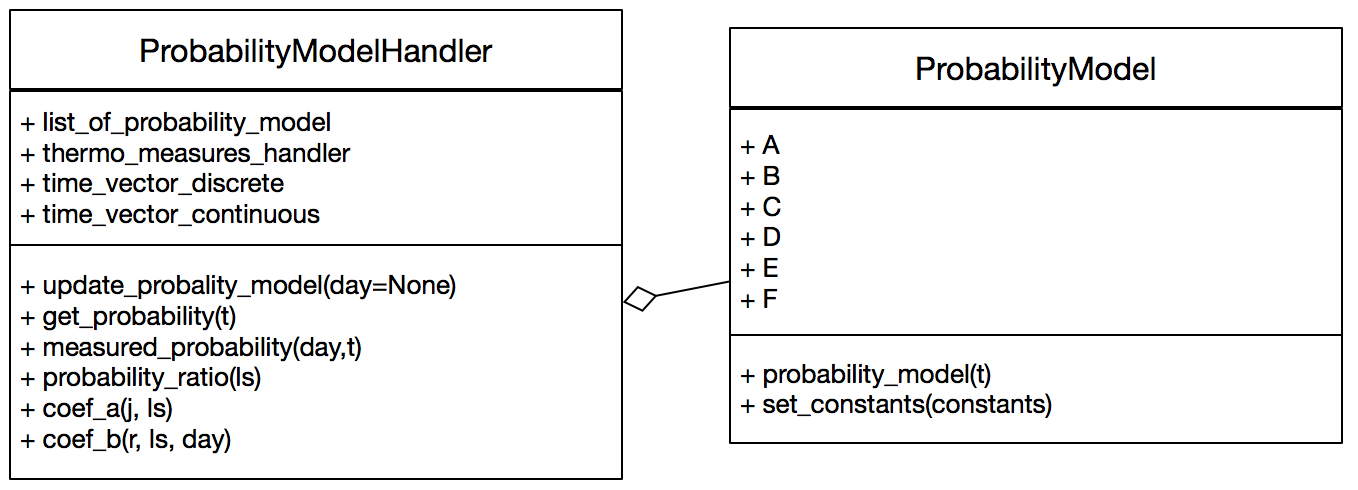
\includegraphics[width=0.75\textwidth]{images/Probability_class_diagram.png}
\caption{Diagrammes des classes \texttt{ProbabilityModel} et \texttt{ProbabilityModelHandler}}
\label{probability_class}
\end{figure}

%TODO : GRAPHIQUE

\subsubsection{Récupération des données et gestion temporelle}
Après une réflexion concernant la distribution temporelle des modèles, il est apparu que le meilleur compromis entre confort d'utilisation et simplicité d'implémentation est de générer un modèle par jour de la semaine. En effet, il est plausible d'estimer que le rythme de vie de l'utilisateur, et donc sa fréquence de présence, est répétitif selon le jour de la semaine. Toutefois, en envisageant que ça ne soit pas le cas, le modèle resterait fonctionnel, il convergerait juste moins rapidement vers la courbe optimale.\\

Afin de regrouper suffisamment de données de présence et de leur donner un sens d'un point de vue statistique, les 24 heures d'une journée ont été discrétisées en 96 éléments\footnote{Ces éléments représentent les $t_{i}$ présentés dans la section \ref{proba_math}.} d'un quart d'heure. En effet, sans cette opération, il serait stochastiquement impossible que deux mesures soient prises le même jour de la semaine précisément à la même heure\footnote{L'heure est encodée au format EPOCH dans la base de données et comporte donc 6 chiffres après la virgule.}. De ce fait, une méthode récupérant les données encodées un jour de la semaine et appartenant au quart d'heure considéré a été codée dans le module \texttt{Data}. La suite de l'implémentation repose sur les données qu'elle récupère.

\subsubsection{Résolution}

\texttt{ProbabilityModelHandler} possède deux méthodes principales : \textit{update\_probality\_model}, qui permet de mettre à jour les coefficients du polynôme de probabilité afin de constamment pouvoir approcher la réalité un maximum. Cette méthode a donc pour objectif de résoudre le système \ref{proba_system} afin d'en déduire les constantes \textit{A B C D E F}. La classe contient également \textit{get\_probabiblity} afin de récupérer la probabilité qu'il y ait quelqu'un à un instant donné. Cette méthode à pour but de \og lire le graphique \fg dessiné par la fonction de probabilité de présence. Cette dernière valeur sera ensuite comparée avec un seuil pour déterminer si la pièce doit être chaude pour cette heure là où non.\\

\section{Prédiction du temps de chauffe}

\subsection{Introduction}

Il est essentiel de pouvoir déterminer le temps exact nécessaire pour chauffer une pièce afin de conserver un confort maximum d'utilisation. Comme mentionné dans la section précédente, l'objectif est d'avoir une pièce chauffée lorsque la valeur de la probabilité de présence passe une valeur seuil. Il apparaît vite que \og simplement \fg enclencher le chauffage lorsque la fonction passe ce seuil n'est pas la manière optimale de procéder.\\

Une prédiction du temps de chauffe propre à chaque pièce doit donc être réalisée. Cette opération systématique est donc réalisée à partir de l'algorithme suivant. Il aura pour objectif de déterminer le temps $t$ nécessaire pour chauffer une pièce d'une température $T_0$ à une température $T_f$.\\

Cette manière de procéder permet deux grands avantages :\\
\begin{itemize}
\item Ne pas devoir utiliser d'équations de chaleur prenant en compte les pertes thermiques de la pièce
\item Ne demande à l'utilisateur de n'effectuer aucune manipulation
\end{itemize}

L'algorithme de prédiction de présence travaillera donc en décalage, si le temps de chauffe est : $t_c$, alors le programme analysera la possibilité d'une présence à $t + t_c$ afin que le chauffage aie le temps de chauffer la pièce.\\

\subsection{Calcul et optimisation des constantes du contrôleur PID}
\label{opti_pid}

Le dispositif pouvant être théoriquement installé dans n'importe quelle pièce et actionner des chauffages de puissances différentes, il doit être capable de calculer l'ouverture optimale de la vanne, et donc par extension les constantes du régulateur PID. 
\subsubsection{Modélisation mathématique}
Du point de vue du PID, un accroissement de température de $t_{0}$ à $t_{k}$ s'exprime :
\begin{equation}
\label{accroissement_temp}
\Delta T = T(t_{k}) - T(t_{0}) = \int_{t_0}^{t_k} PID(t) dt \Leftrightarrow T(t_{k}) = T(t_{0}) + \int_{t_0}^{t_k} PID(t) dt
\end{equation}
En effet, il n'est pas nécessaire de tenir compte des caractéristiques thermodynamiques de la pièce car le PID ne doit pas modéliser de comportement thermique. Les effets de ces paramètres sont pris en compte dans ses trois constantes. \\
Si on considère deux instants proches $t_i$ et $t_{i-1}$, il est acceptable de considérer que l'équation \ref{accroissement_temp} peut être approchée par :
\begin{equation}
T(t_i) \approx T(t_{i-1})+PID(t_{i-1}) * (t_i - t_{i-1})
\end{equation}
Le but poursuivi par le régulateur PID est d'atteindre une température cible $T_T$ le plus rapidement possible et ensuite de la maintenir. En d'autres mots, il minimise en permanence la différence entre la température actuelle et la température visée. L'expression à minimiser vaut :
\begin{equation}
\sum_{i=1}^{n} (T(t_{i-1})+PID(t_{i-1}) * (t_i - t_{i-1}) - T_{T}(t_i))^2
\end{equation}
Ce qui donne, en injectant l'expression d'un PID :

\begin{equation}
\sum_{i=1}^{n} (T(t_{i-1})+ K_p e(t_{i-1}) + K_i \int_{t_{0}}^{t_{i-1}} e(t)dt + K_d\frac{d}{dt}e(t_{i-1})* (t_i - t_{i-1}) - T_{T}(t_i))^2
\end{equation}

En dérivant trois fois l'équation par rapport aux constantes $K_p$, $K_i$ et $K_d$, de la même manière que pour la prédiction de présence, on obtient le système suivant :\\

\begin{equation}
\label{systeme_nul}
\left\{
\begin{aligned}
& \sum_{i=1}^{n} e(t_{i-1}) * (T(t_{i-1})+ K_p e(t_{i-1}) + K_i \int_{t_{0}}^{t_{i-1}} e(t)dt + K_d\frac{d}{dt}e(t_{i-1})* (t_i - t_{i-1}) - T_{T}(t_i)) = 0\\
& \sum_{i=1}^{n} \int_{t_{0}}^{t_{i-1}} e(t)dt * (T(t_{i-1})+ K_p e(t_{i-1}) + K_i \int_{t_{0}}^{t_{i-1}} e(t)dt + K_d\frac{d}{dt}e(t_{i-1})* (t_i - t_{i-1}) - T_{T}(t_i)) = 0\\
& \sum_{i=1}^{n} \frac{d}{dt}e(t_{i-1})* (t_i - t_{i-1}) * (T(t_{i-1})+ K_p e(t_{i-1}) + K_i \int_{t_{0}}^{t_{i-1}} e(t)dt + K_d\frac{d}{dt}e(t_{i-1})* (t_i - t_{i-1}) - T_{T}(t_i)) = 0\\
\end{aligned} \right.
\end{equation}

A nouveau, comme pour la modélisation de la probabilité de présence, les valeurs des constantes qui minimisent cette différence sont le résultat du système \ref{systeme_nul}.\\

\subsubsection{Implémentation}
La classe \texttt{PIDHandler} présentée à la section \ref{pid_section} est utilisée pour résoudre ce système. Une méthode principale \texttt{update\_pid\_model} fait appel à de nombreuses fonctions qui sont utilisées afin de générer les coefficients des matrices à résoudre, et des algorithmes d'analyse numérique ont été implémentés\footnote{Afin de mettre en place une résolution propre du calcul intégral et différentiel.}\cite{ananum}.\\
Ce calcul fait appel à une fonction agissant sur la base de données afin de récupérer toutes les entrées reçues le jour où une optimisation est lancée\footnote{Cette classe a été pensée de manière à exécuter ses méthodes une fois par jour.} C'est dans cette optique qu'une colonne  supplémentaire, la \og target\_temp \fg, y a été ajoutée.


\subsection{Calcul des constantes thermodynamiques}

Le but de cette section est d'étudier le comportement thermique d'une pièce. Pour ce faire, le code doit analyser ses caractéristiques thermodynamiques.

\subsubsection{Modélisation mathématique}
En définissant $P_f$ et $P_d$, respectivement les puissances fournies et dissipées dans la pièce considérée, il est possible de modéliser l'évolution de la température comme suit:
\begin{equation}
T(t) = T(t_0) + \int_{t_0}^{t} P_{f}(\tau) d\tau - \int_{t_0}^{t} P_{d}(\tau) d\tau
\end{equation}
$P_f$ peut être exprimée comme un coefficient\footnote{Correspondant à la puissance maximale du chauffage.} modulé par la valeur du PID. $P_d$ quant à elle, s'apparente à la loi de Fourier pour les pertes de chaleur aux travers de parois\cite{haelti}. Elle s'exprime donc comme une constante thermique\footnote{Equivalente à la tendance qu'a l'habitation à dissiper sa chaleur.} multipliée par la différence de température entre la pièce et l'extérieur. En tenant compte de ces relations, on obtient :
\begin{equation}
\label{thermo}
T(t) = T(t_0) + P_{max}\int_{t_0}^{t} PID(\tau) d\tau - \sigma \int_{t_0}^{t} (T(\tau) - T_{ext}(\tau) d\tau
\end{equation}
Le but de cette modélisation est de déterminer ces deux constantes. Pour ce faire, il faut répéter la prise de mesures deux fois. Dès lors un système de deux équations est obtenu.\\

\subsubsection{Implémentation}

Ce module n'a été implémenté que basiquement, et ne présente pas de structure claire à présenter. Toutefois, cette classe accède à la base de données afin de récolter les données brutes nécessaires au calcul des coefficients du système. Tout comme les autres codes intelligents, il a été pensé de telle sorte à ce s'exécuter régulièrement afin de s'adapter si des changements d'environnement ont lieu.
\subsection{Conclusion}
Ces nombreux calculs ont pour but de permettre au serveur de prévoir le temps que va mettre une pièce pour atteindre une température, en connaissant les températures actuelle et extérieure. Pour ce faire, il interroge le \texttt{PID}, qui en permanence évalue cette valeur. Ce dernier est en mesure de le faire car il connaît le modèle thermique de la pièce dans laquelle le Remote Device auquel il est lié est situé. Il simule un ordre de chauffe, et renvoie le temps $\Delta t$ qu'il faut pour atteindre la température désirée.\\

Ce module n'est pas encore fonctionnel, et n'a donc pas été testé entièrement. Le calcul des constantes du PID ne donne pas de résultats corrects. Il a été envisagé d'appliquer une méthode tout à fait différente, celle de Ziegler-Nichols\cite{zieg}. Elle n'a toutefois pas été retenue dans un premier temps car son implémentation semblait trop complexe. Cependant, elle semble à présent être celle à utiliser si il fallait rendre le code fonctionnel.

\section{Fonctionnement du code intelligent}

Des éléments intelligents sont présents dans deux Threads. Cette section va présenter comment le serveur va les utiliser.

\subsection{Thread principal}
Dans la classe \texttt{ThermoServer}, une méthode principale, \texttt{magic\_function}, tourne en permanence. Celle-ci, en plus de s'occuper de la récolte et du stockage des données pour chaque remote device, va évaluer la nécessité de chauffer la pièce dans laquelle il se situe. Pour se faire, elle utilise le modèle de probabilité du jour ainsi que le temps de chauffe fourni par les simulations du \texttt{PID}. \\

Lorsque le serveur évalue la probabilité de présence en un instant, il la compare à une valeur seuil, la \og Trigger value \fg\footnote{Conventionnellement, cette valeur vaut 0,5.}. Si celle-ci est inférieure à la probabilité actuelle, un ordre de chauffe est envoyé. Ceci pose un problème. En effet, cette manière de faire est en retard, car l'activation des radiateurs a seulement lieu au moment où un utilisateur est susceptible d'arriver. C'est pour celà qu'il faut considérer le temps de chauffe de la pièce.\\
Si on considère $t$, l'instant présent, et $\Delta t$, le temps de nécessaire pour atteindre la température visée, la probabilité à considérer sera celle-ci : 
\begin{equation}
p(t + \Delta t)
\end{equation}

\subsection{Thread d'optimisation}
En parallèle, un thread de calcul et d'optimisation de toutes les constantes évoquées dans ce chapitre sera exécuté une fois par jour. De cette manière, le code s'adaptera si des changements interviennent dans les habitudes des utilisateurs ou dans les caractéristiques thermodynamiques d'une pièce\footnote{Changement d'emploi, horaires différents, nouvelle isolation, installation de double-vitrage, nouveaux chauffages, déménagement,...}.


%\newpage
%--------------------------------------------------------------------------------------
%	TESTS
%--------------------------------------------------------------------------------------

%\chapter{Tests}

%Des tests ont été réalisés afin de terminer la validité de toutes les implémentations. Tant celles des périphériques de l’Arduino que du Raspberry pi. Ces tests permettent de vérifier que le dispositif fonctionne normalement dans un maximum de conditions différentes. Le tout dans le but d’améliorer le thermostat et de vérifier son bon fonctionnement dans différentes utilisations. Le principe du test est d’effectuer une dizaine de fois la même opération et de vérifié que le résultat obtenu est bien celui attendu.\\

%\section{Tests sur les \og remotes devices \fg}

%Comme mentionné précédemment, les \og remotes devices \fg sont composés de plusieurs capteurs différents. Les différents tests à réaliser concerneront : Le capteur de présence, le thermistance, le module wifi, et la réunion de ces trois modules.\\

%\subsection{Validation du capteur de présence}

%Ce capteur de présence sera testé à l’aide du code fourni en annexe ??. Il a été placé dans une pièce initialement vide et différentes personnes sont rentrées et sorties. Des déplacements à courte distance ont également été effectué afin d'échantillonner la distance d'utilisation. La distance est finalement apparue comme sans effet sur les tests.\\ 

%\subsection{Validation du modèle de la thermistance} 

%Ce thermistance a été testé dans diverses conditions, tant intérieures qu’extérieures afin d’obtenir une vaste plage de températures dans lequel sa validité pourrait  confirmée à l'aide d'un autre thermomètre. Ces tests informels ont donc confirmés le fonctionnement de cet fonction du remote device.\\

%to do: les 2 références aux annexes à remplir, le tableau de donnée à remplir??

%RETODO :  Je n'ai pas réussi a faire fonctionner le raspberry et l'arduino chez moi,
%RETODO : Je pensais que ces codes sera placés en annexes ? Ce n'est pas le cas ?
%RERETODO : Pas de code dans le rapport, espèce d'insouciant!! :p (Steph), au pire on peut les mettre dans les délivrable dans un dossier test. 
%RERETODO: (soufiane) Alors on supprime les tableaux?? Je viens de voir que les tests ont pas été fait et demain je suis pas chez moi avant tard le soir....on m'a pas dit qu'il fallait que je fasse les tests c'est dommage
%\section{Tests sur le thermostat central}

%\subsection{Validation du serveur}
%to do: y a rien pour ca? Meme pas dire qu'on va le faire au deuxième quadri?
%RETODO : Done

%Des tests informels ont été réalisés afin de tester le fonctionnement du serveur. Le remplissage de la base de données implique que le serveur est opérationnel mais une méthode de test plus rigoureuse envisageant un maximum de cas possible sera rédigée et effectuée lors du deuxième quadrimestre.\\

%\subsection{Validation de la base de donnée}

%La base de donnée doit être soumis à de nombreux cas de figures afin de déterminer sa validité. Le premier test est de lancer le serveur sur le raspberry avec la base de donnée connectée à un Arduino et de lui demander de stocker les données récoltées par le Raspberry. Ce test fut effectué avec succès, ce qui confirme que la méthode \og add\_entry \fg et \og create\_table \fg fonctionne.\\

%Une autre méthode à tester est  \og table\_already\_exists \fg et \og recover\_table \fg. Ce test consiste à débrancher le Raspberry durant son fonctionnement afin de simuler une coupure de courant et de le relancer par après afin de voir si les données qu'il collectera à nouveau sur le même Arduino seront insérées dans la même table oui ou non. Ce test fut concluant également.\\

%\section{Tests à effectuer à posteriori}

%Tous ces tests permettent d'attester du fonctionnement effectif de la base de donnée, du serveur, de l'arduino, du capteur de présence, etc. Mais ils ne constituent pas en réalité d'un protocole de test en bonne et due forme. Une méthode de test bien plus rigoureuse, consistant. De plus, des modules tels que la base de donnée prendront une forme nouvelle, il sera donc nécéssaire d'adapter les tests réalisés à la nouvelle structure.\\



%to do: repréciser que puisqu'on va le changer au deuxième quadri et que donc on va faire des tests spécifiques aux nouvelles bases de données non? Faudrait aussi parler que nos tests seront plus rigoureux aux deuxième quadri pour l'ensemble des modules et que ca c'est juste des tests pour voir si ca marche

%RETODO : done

\newpage
%----------------------------------------------------------------------------------------
%	FONCTIONNEMENT DE GROUPE
%----------------------------------------------------------------------------------------

\chapter{Stratégie de tests et validation}

Une fois l'implémentation des codes finalisée et malgré leur fonctionnement apparent, il est indispensable de réaliser deux tâches.\\

La première tâche consiste à mettre sur pied une stratégie de tests et d'essayer toute une série de scénario pour voir comment réagissent le thermostat individuel et le thermostat central à ces différents stress tests. Est ce que la gestion des exceptions est opérationnelle? Que se passe-t-il si le serveur central s'éteint brutalement? Et qu'en est il des données envoyées si le matériel est défaillant? Autant de questions auxquelles les tests doivent pouvoir répondre.\\ 

D'un autre côté, il faut également que le thermostat puisse être évalué par des critères objectifs. Il faut donc pour cela développer des indicateurs de qualité qui permettent de disposer d'arguments forts sur les avantages ou les désavantages du système développé.\\

Enfin, il est à noter que suite à des événements indépendants de notre volonté (Le module wifi a été défaillant pendant plusieurs semaines malgré son remplacement.), il n'a pas été possible de tester et observer des résultats pour tout ce qui devait être testé. Néanmoins, il a été décidé de quand même exposer la réflexion du groupe sur qui a voulu être implémenté comme tests.\\

\section{Stratégie de tests}
Chaque test sera explicité selon deux aspects, ce qui fut testé et les résultats qui furent attendus et/ou observés.

%A tester: hardware, arduino: connexion, envoie de requetes

% Serveur central: connexion arduino, connexion bdd,

%bdd

\begin{itemize}[noitemsep]
\item Les composants du thermosat individuel: la prise de température par la thermistance, le détecteur de présence, l'ouverture des vannes de l'environnement physique, l'envoi ou la réception de requêtes au serveur central par le module WiFi. Tous ces tests ont été concluants. Notons que pour la thermistance, les résultats obtenus ont été comparé à la température obtenue par l'environnement physique. \textit{(Notons tout de même une légère exception suite à la défectuosité du module Wi-fi, mais il s'avère que la source d'erreur se trouve être le module lui même et non le code)}\\

\item Le serveur central: la connexion à la base de donnée, l'envoi de requêtes, la réception de requêtes d'enregistrement du thermostat individuel et de l'environnement furent testés. La création d'une base de donnée si elle est inexistante et l'utilisation d'une base de donnée si elle existe également. Les tests ont tous été concluants.\\


\item Le régulateur de température (PID) sans initialisation automatique des constantes: l'objectif était de tester si le régulateur PID fonctionnait parfaitement si on déterminait expérimentalement les constantes du PID. Puisque le module WiFi ne fonctionnait déjà plus à ce moment là, il a été décidé de créer un script pour simuler un environnement (Voir annexe. Le résultat est que le PID permettait d'atteindre la valeur consigne et de stabiliser la température autour de cette valeur (voir Figure \ref{PID}). Une remarque importante doit être signalée sur le simulateur. En effet, le gain en température a été codé comme étant proportionnel à l'ouverture de la vanne et la perte proportionnelle à la différence entre la température mesurée et la température extérieure. Il ne convient donc pas de tirer de pertinence sur la lecture du temps passé en abscisses car elles dépendent de ces coefficients de proportionnalité. Notons enfin que la température initiale vaut 10 et la valeur consigne 20..\\

\begin{figure}[h]
\centering
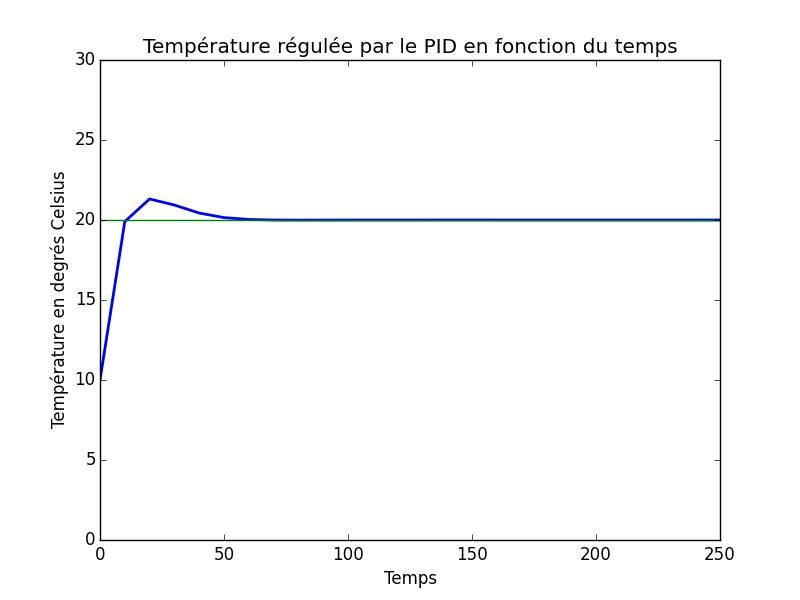
\includegraphics[width=0.5\textwidth]{images/pidSimul.jpg}
\caption{Résultat du PID par simulation}
\label{PID}
\end{figure}

% Mettre simulateur en annexe?

\item Le régulateur de température (PID) avec initialisation automatique des constantes: l'objectif était de tester si le régulateur PID était capable d'initialiser automatiquement ses constantes. Malheureusement, force est de constater que les résultats avec le simulateur n'étaient pas concluants. Un problème de modélisation théorique semble être à l'origine du problème.\\

%Graphe?

\item Modèle prédictif de présence: l'objectif était de voir si le serveur central était capable d'observer une courbe de probabilité à partir de données qui lui seraient envoyées. Là encore, le problème du module WiFi ne nous a pas permis de tester directement le code. Il a donc à nouveau été question d'utiliser un simulateur de données afin d'observer les résultats obtenus. Les résultats ont été concluants. La modélisation par interpolation polynomiale de degré 5 permet bien d'obtenir une courbe de probabilité (voir Figure \ref{proba1} et \ref{proba2}). Il peut être utile de signaler que lorsque la probabilité de présence n'est pas comprise dans l'intervalle [0,1], elle est automatiquement ramenée à l'une de ces deux valeurs dans le code.\\

\begin{figure}[h]
\centering
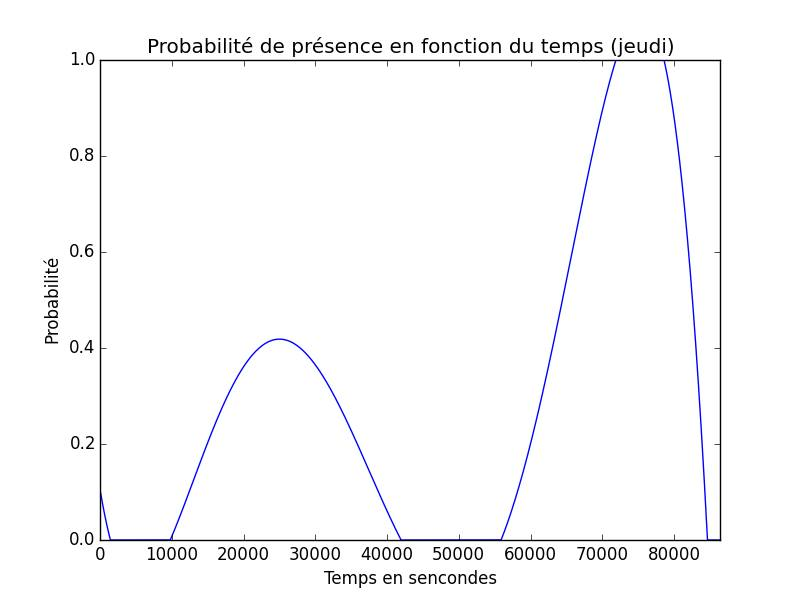
\includegraphics[width=0.5\textwidth]{images/proba2.jpg}
\caption{Résultat du modèle de prédiction par simulation - Jeudi}
\label{proba2}
\end{figure}

\begin{figure}[h]
\centering
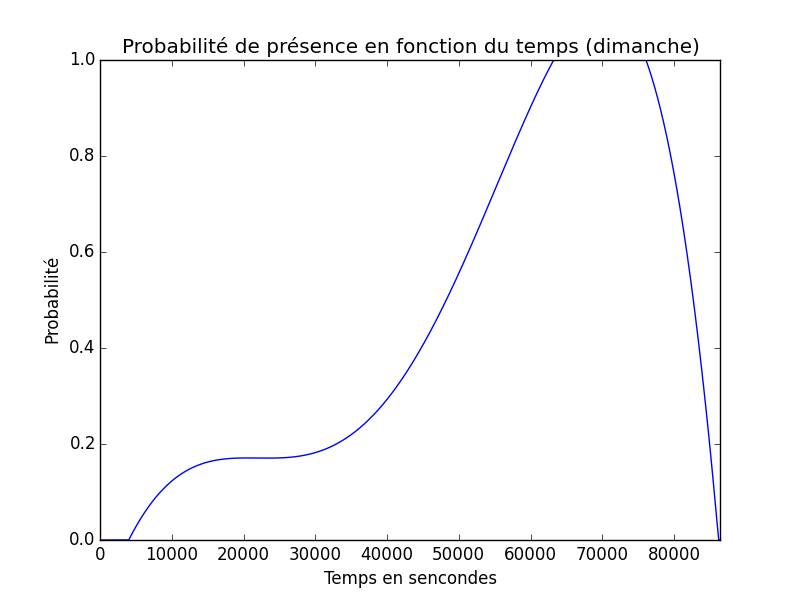
\includegraphics[width=0.5\textwidth]{images/proba1.jpg}
\caption{Résultat du modèle de prédiction par simulation - Dimanche}
\label{proba1}
\end{figure}

\end{itemize}

\section{Validation du modèle}

Pour la validation du modèle, quatre questions seraient intéressantes à analyser en se positionnant en tant qu'utilisateur du thermostat intelligent. Il a en effet toutes les chances de se poser les questions suivantes :\\

\begin{enumerate}
\item L'intelligence du code permet-il de prédire efficacement la présence de l'utilisateur?\\
\item Lorsque qu'une valeur consigne doit être atteinte, à quelle vitesse cette valeur est-elle atteinte?\\
\item Une fois cette valeur atteinte, le régulateur est-il assez performant pour maintenir une température stable et ne pas osciller ?\\
\item Quel est le coût énergétique de ce régulateur en comparaison au "On/Off" algorithme?\\

\end{enumerate}

Étant donné les problèmes du module WiFi évoqué dans la section "Stratégie de test", il n'a été possible que d'évoquer les indicateurs tels qu'ils auraient été implémenté si cela avait été possible. Les solutions auraient respectivement été:

\begin{enumerate}
\item Le modèle est censé prédire une présence à chaque seconde pendant 24h. Il suffit de comptabiliser le nombre de fois où il a préchauffé une pièce alors qu'il ne fallait pas et le nombre de fois où il n'a pas préchauffé une pièce alors que quelqu'un arrivait et on divise la somme de ces résultats par le nombre d'observations totales faites sur une journée. Plus cet indicateur est bas et plus le modèle prédictif est bon.\\

\item Il faudrait lancer le programme et de récolter les données à intervalles réguliers afin de connaître le temps nécessaire au thermostat pour atteindre la valeur consigne. Il pourrait également être intéressant de connaitre la variation de ce temps de chauffe lorsque chaque constante du PID est modifiée.\\

\item Une méthode utile serait de calcul sommer tous les écarts de température et donc d'intégrer cette fonction au carré\footnote{Afin d'éviter les annulations d'erreur} sur tout l'intervalle où la température est sensée ne plus varier. Un algorithme stable devrait avoir une valeur de l'intégrale proche de 0.\\

\item Une possibilité serait de considérer l'ouverture moyenne de la vanne au cours du temps pour les deux régulateurs. Cela en comptant que le fait d'allumer le chauffage consomme également plus d'énergie \textit{(Pompage)}.\\

\end{enumerate}

\chapter{Fonctionnement de groupe}

	Afin d’atteindre les objectifs du projet le plus rapidement et le plus efficacement possible, il était important d’établir une bonne organisation du travail en groupe afin de maximiser la productivité du groupe et de répartir la quantité de tâches à effectuer par chacun de manière équitable. Quelques outils ont donc été mis en place dès la première semaine dans cette optique.\\

	Pour commencer, le plus important était de définir comment les informations transiteraient. Un groupe privé sur Facebook a été choisi pour la communication informelle en dehors des réunions, l’avantage étant de pouvoir conserver un historique de ces conversations. Le transfert des documents, codes, parties de rapport,... s’effectue quant à lui via une Dropbox qui permet d'archiver et de partager tous ces fichiers de façon simple et efficace. Il a également été décidé que le rapport serait rédigé en \LaTeX ~sur \og Overleaf\footnote{\url{https://www.overleaf.com/}} \fg, cette plate-forme permettant la modification en temps réel du document par tous les membres de l’équipe.\\

	La fréquence des réunions fut fixée au rythme de deux par semaines. Une avec le tuteur du projet afin de le tenir au courant des avancées réalisées lors de l’autre réunion qui concerne uniquement les membres du groupe. Lors de ces rencontres hebdomadaires, chacun se doit de comprendre les avancée exposées par les autres membres du groupe afin d’obtenir des connaissances homogènes dans tous les domaines. Cette fréquence permet de ne pas oublier de travailler chaque semaine sur le projet. Il arrive que des réunions supplémentaires soient organisées en équipe lorsque le besoin s’en fait sentir ou qu’une deadline approche.\\

	Ces réunions se tiennent, sauf cas de force majeure, à la Bibliothèque des Sciences et Techniques de l’ULB, principalement pour des raisons de proximité. Durant ces réunions, un membre est désigné et joue le rôle de secrétaire et d’animateur. La fusion de ces deux rôles a été décidée en raison de la taille du groupe. La tâche de de cette personne est d’envoyer l’ordre du jour aux autres membres au moins 24 heures avant la réunion, de l’animer ensuite et d’en rédiger le procès-verbal par après. Ce poste est attribué à une autre personne toutes les deux semaines sur base volontaire afin de ne surcharger personne de travail.\\
    
\newpage

%--------------------------------------------------------------------------------------
%	PERSPECTIVES D'EVOLUTION
%--------------------------------------------------------------------------------------

\chapter{Perspectives d'évolution}

Beaucoup d'hypothèse simplificatrice ont été faites jusqu'ici. Il est donc intéressant d'envisager des moyens de les surmonter.

\subsection*{Dans l'implémentation} % TODO: quoi d'autre comme problème?
\paragraph{L'identification des remote device}: Le serveur gérant les remote device n'a pas de moyen infaillible de les identifier sur le long terme (entre plusieurs connexion-déconnexion). Les informations d'indentification sont un nom qui est attribué par le serveur (ou par l'utilisateur par l'intermédiaire du serveur) et une addresse ip. Aucune des ces deux données n'est assurément fixe après un redémarrage du device. Le moyen le plus simple de palier à ce problème serait de se baser sur un identifiant statique et unique (l'adresse MAC du module wifi d'un device par exemple).

\subsection*{Dans les modèles prédictifs}
\paragraph{Types de données disponibles}: Une des contraintes principale de ce projet est la limitation des types de mesure prise par "thin thermostat" (type de remote device).Cela contraint les modèle prédictif: par exemple l'utilisation des méthodes de prédiction de présence basée sur la géolocalisation des utilisateurs est bien plus précise. La température intérieure et la consommation énergétique dépendent également de bien d'autres données que de la température intérieur et extérieur et de l'ouverture d'une vanne, la luminosité, l'ouverture des porte et fenêtre et d'autres élément peuvent être pris en compte pour affiner et corrigé les modèle.

\paragraph{Définition du confort}: En prenant une définition du confort prenant en compte plus d'élément permettrait de rendre le thermostat plus apte à satisfaire son utilisateur. Des éléments comme cité dans la sous-section \ref{critere_intelligence} du chapitre 5 pourraient être insérées au thermostat.

\subsection*{Dans l'interaction avec l'utilisateur}

\paragraph{Interface graphique}: L'ajout d'une interface graphique permettant à l'utilisateur de pouvoir interagir plus aisément avec l'appareil, en modifiant la température visée, l'humidité, etc à tout instant sur un site internet, une application, etc.

\paragraph{L'accès aux informations}: L'utilisateur pourrait également avoir un contrôle plus grand sur sa consommation en visualisant les heures d'ouverture de la vanne, en ayant la possibilité également de synchroniser son agenda avec le thermostat afin d'être sur que le chauffage ne se mette pas en route (Dans le cas des vacances à l'étranger par exemple). 

\newpage
%--------------------------------------------------------------------------------------
%	CONCLUSIONS
%--------------------------------------------------------------------------------------

\chapter{Conclusion}

La conception et la visualisation des demandes du projet était la première étape clé du processus de fabrication du thermostat intelligent. L'utilisation du diagramme présenté en Annexe \ref{dia_complet} était le moyen le plus efficace de se représenter l'objectif final. La réalisation du câblage des différents composants a été assez rapidement effectué, tout comme l'implémentation de l'Arduino, bien que parfois celle-ci ait été retardée suite à un manque de matériel. Toutefois, certaines complications ont entraîné plusieurs modifications du câblage de l'Arduino.\\

L'autre partie abordée en parallèle concernait le Raspberry. La création d'un serveur était nécessaire, l'implémentation de celui-ci est telle qu'il permet une plus grande flexibilité que celle exigée par le cahier des charges. En effet, on peut y connecter n'importe quel type de Remote Device. Comme exigé dans le cahier des charges, les communications respectent le protocole HTTP.\\

Un stockage des données était nécessaire afin d'implémenter l'analyse intelligente. Une étude a été menée afin de choisir entre les différentes façon de faire et SQLite a finalement été retenu pour sa légèreté, sa simplicité et sa présence par défaut dans Python. L'implémentation fut sujette à une grosse modification mais respecte aujourd'hui les conventions.\\

L'algorithme de contrôle de la vanne a été implémenté en deux étapes, d'abord un simple \og ON/OFF \fg, suivi par après d'un algorithme intelligent et prédictif, utilisant la base de donnée pour prédire la présence future ou non de l'utilisateur. Un régulateur PID est également implémenté afin de minimiser l'oscillation de la température et de réduire la consommation énergétique.\\

Ces algorithmes ont nécessités la mise en place de modèle mathématiques qu'il a fallu valider par la suite. Ces derniers ont donc fait l'objet de tests tout comme les thermostats individuels, centraux, etc. La plupart de ces tests furent concluants excepté pour l'actualisation des constantes du PID, il s'avère que ce processus souffrirait d'un problème de modélisation.\\

Le fonctionnement du groupe n'a pas nécessite de modifications durant l'année, la répartition du travail était équitable et les réunions hebdomadaires permettaient un suivi régulier du travail effectué. Cette méthode de travail semble être une bonne base pour de futurs projets.\\

Le travail a fournir était assez conséquent et les problèmes rencontré avec le fonctionnement ont considérablement ralenti la bonne marche du projet, mais malgré tout les quatre Milestones ont globalement été complétées. Des améliorations de ce projet sont toutefois possibles comme elles ont été énoncés plus haut.


\newpage

%--------------------------------------------------------------------------------------
%	MEMBRES DU GROUPE
%--------------------------------------------------------------------------------------

\chapter{Membres du groupe}

\begin{minipage}{0.45\textwidth}
\begin{flushleft} 
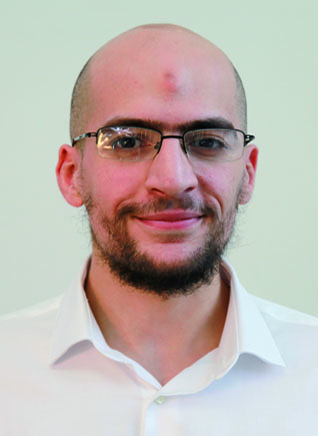
\includegraphics[height=4cm] {photos_membres/Soufiane.jpg}\\
\textsc{Amzur} Soufiane\\
\textsc{000328725}\\
\textsc{soufiane.amz@gmail.com}\\
\end{flushleft}
\end{minipage}
~
\begin{minipage}{0.45\textwidth}
\begin{flushright}
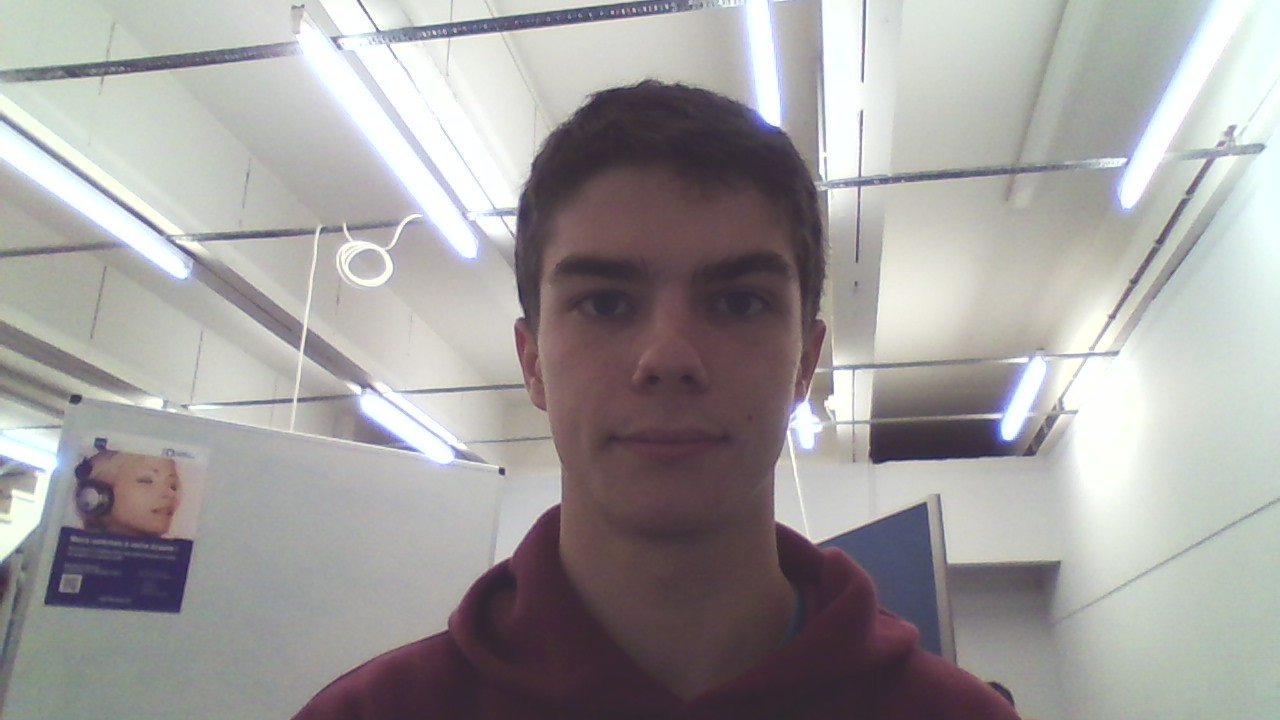
\includegraphics[height=4cm]{photos_membres/Wilson.jpg}\\
\textsc{Daubry} Wilson\\
\textsc{000408780}\\
\textsc{daubry.wilson@gmail.com}\\
\end{flushright}
\end{minipage}

\emph{} \\
\emph{} \\
\emph{} \\
\emph{} \\
\emph{} \\

\begin{minipage}{0.45\textwidth}
\begin{flushleft} 
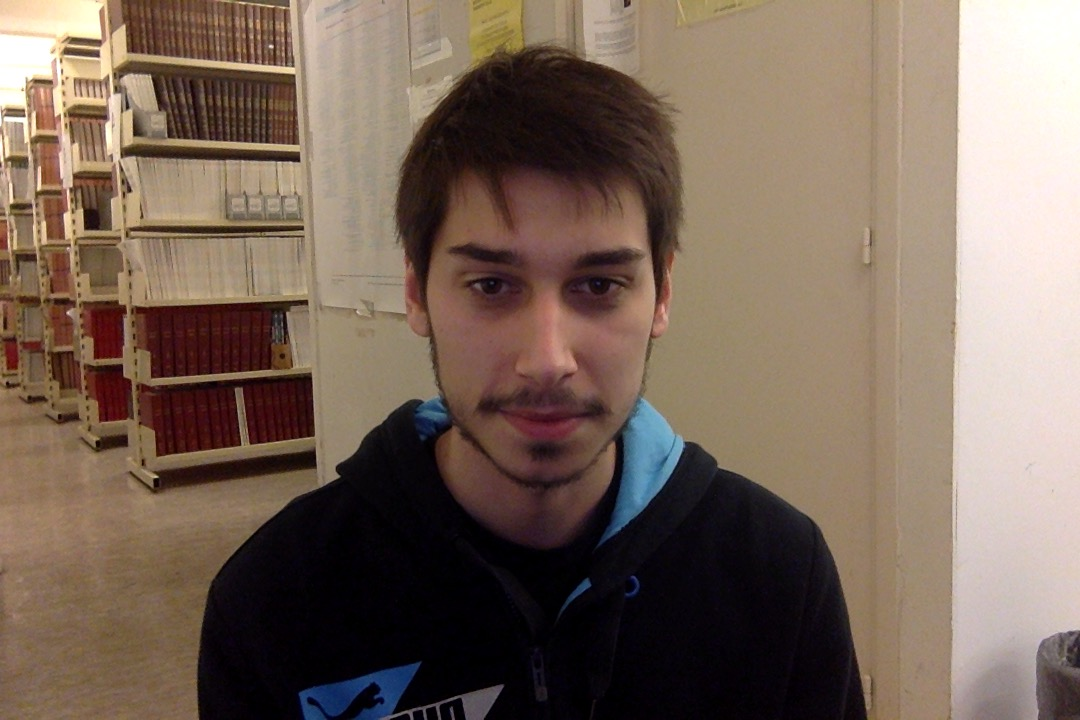
\includegraphics[height=4cm] {photos_membres/Stephane.jpg}\\
\textsc{Sercu} Stephane\\
\textsc{000408643}\\
\textsc{ssercu@ulb.ac.be}\\
\end{flushleft}
\end{minipage}
~
\begin{minipage}{0.45\textwidth}
\begin{flushright}
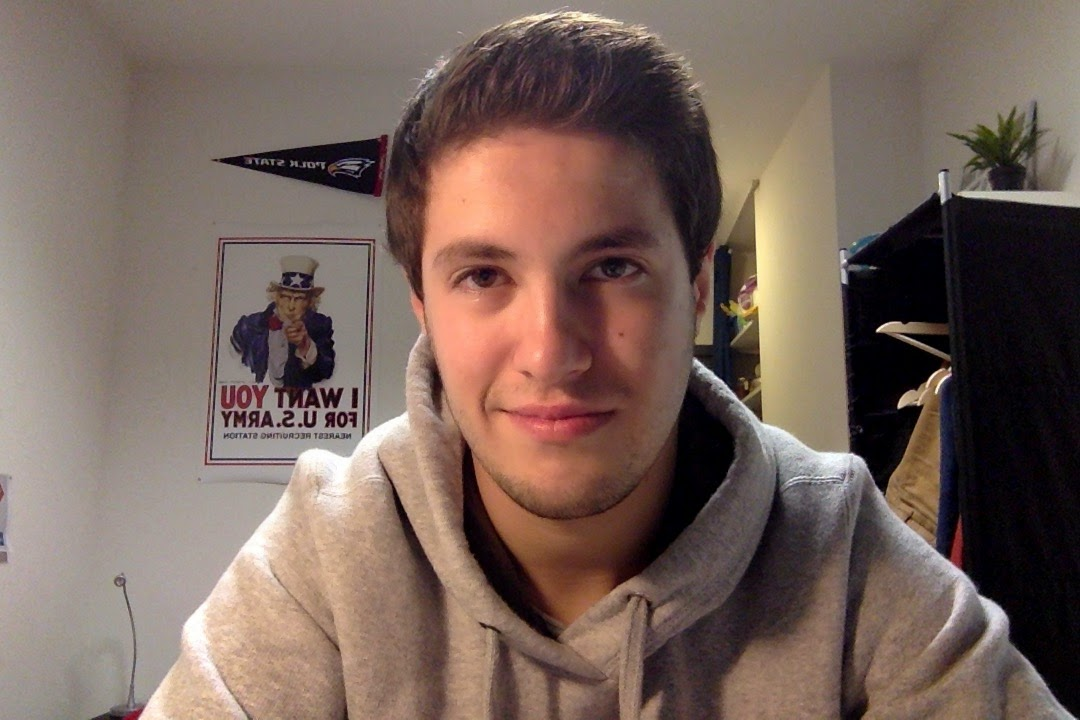
\includegraphics[height=4cm]{photos_membres/Denis.jpg}\\
\textsc{Verstraeten} Denis\\
\textsc{000401967}\\
\textsc{denverst@ulb.ac.be}\\
\end{flushright}
\end{minipage}

\newpage

%to do: ma photo doit etre au mm format que la votre

%RETODO : Prendre nos 4 photos avec le mac de Denis Mais est ce vraiment un probleme ? Ma photo non plus n'a pas les meme dimension

%RERETODO: ok on s'en fout alors lol

\appendix

%======================================================================================
%	ANNEXES
%======================================================================================


%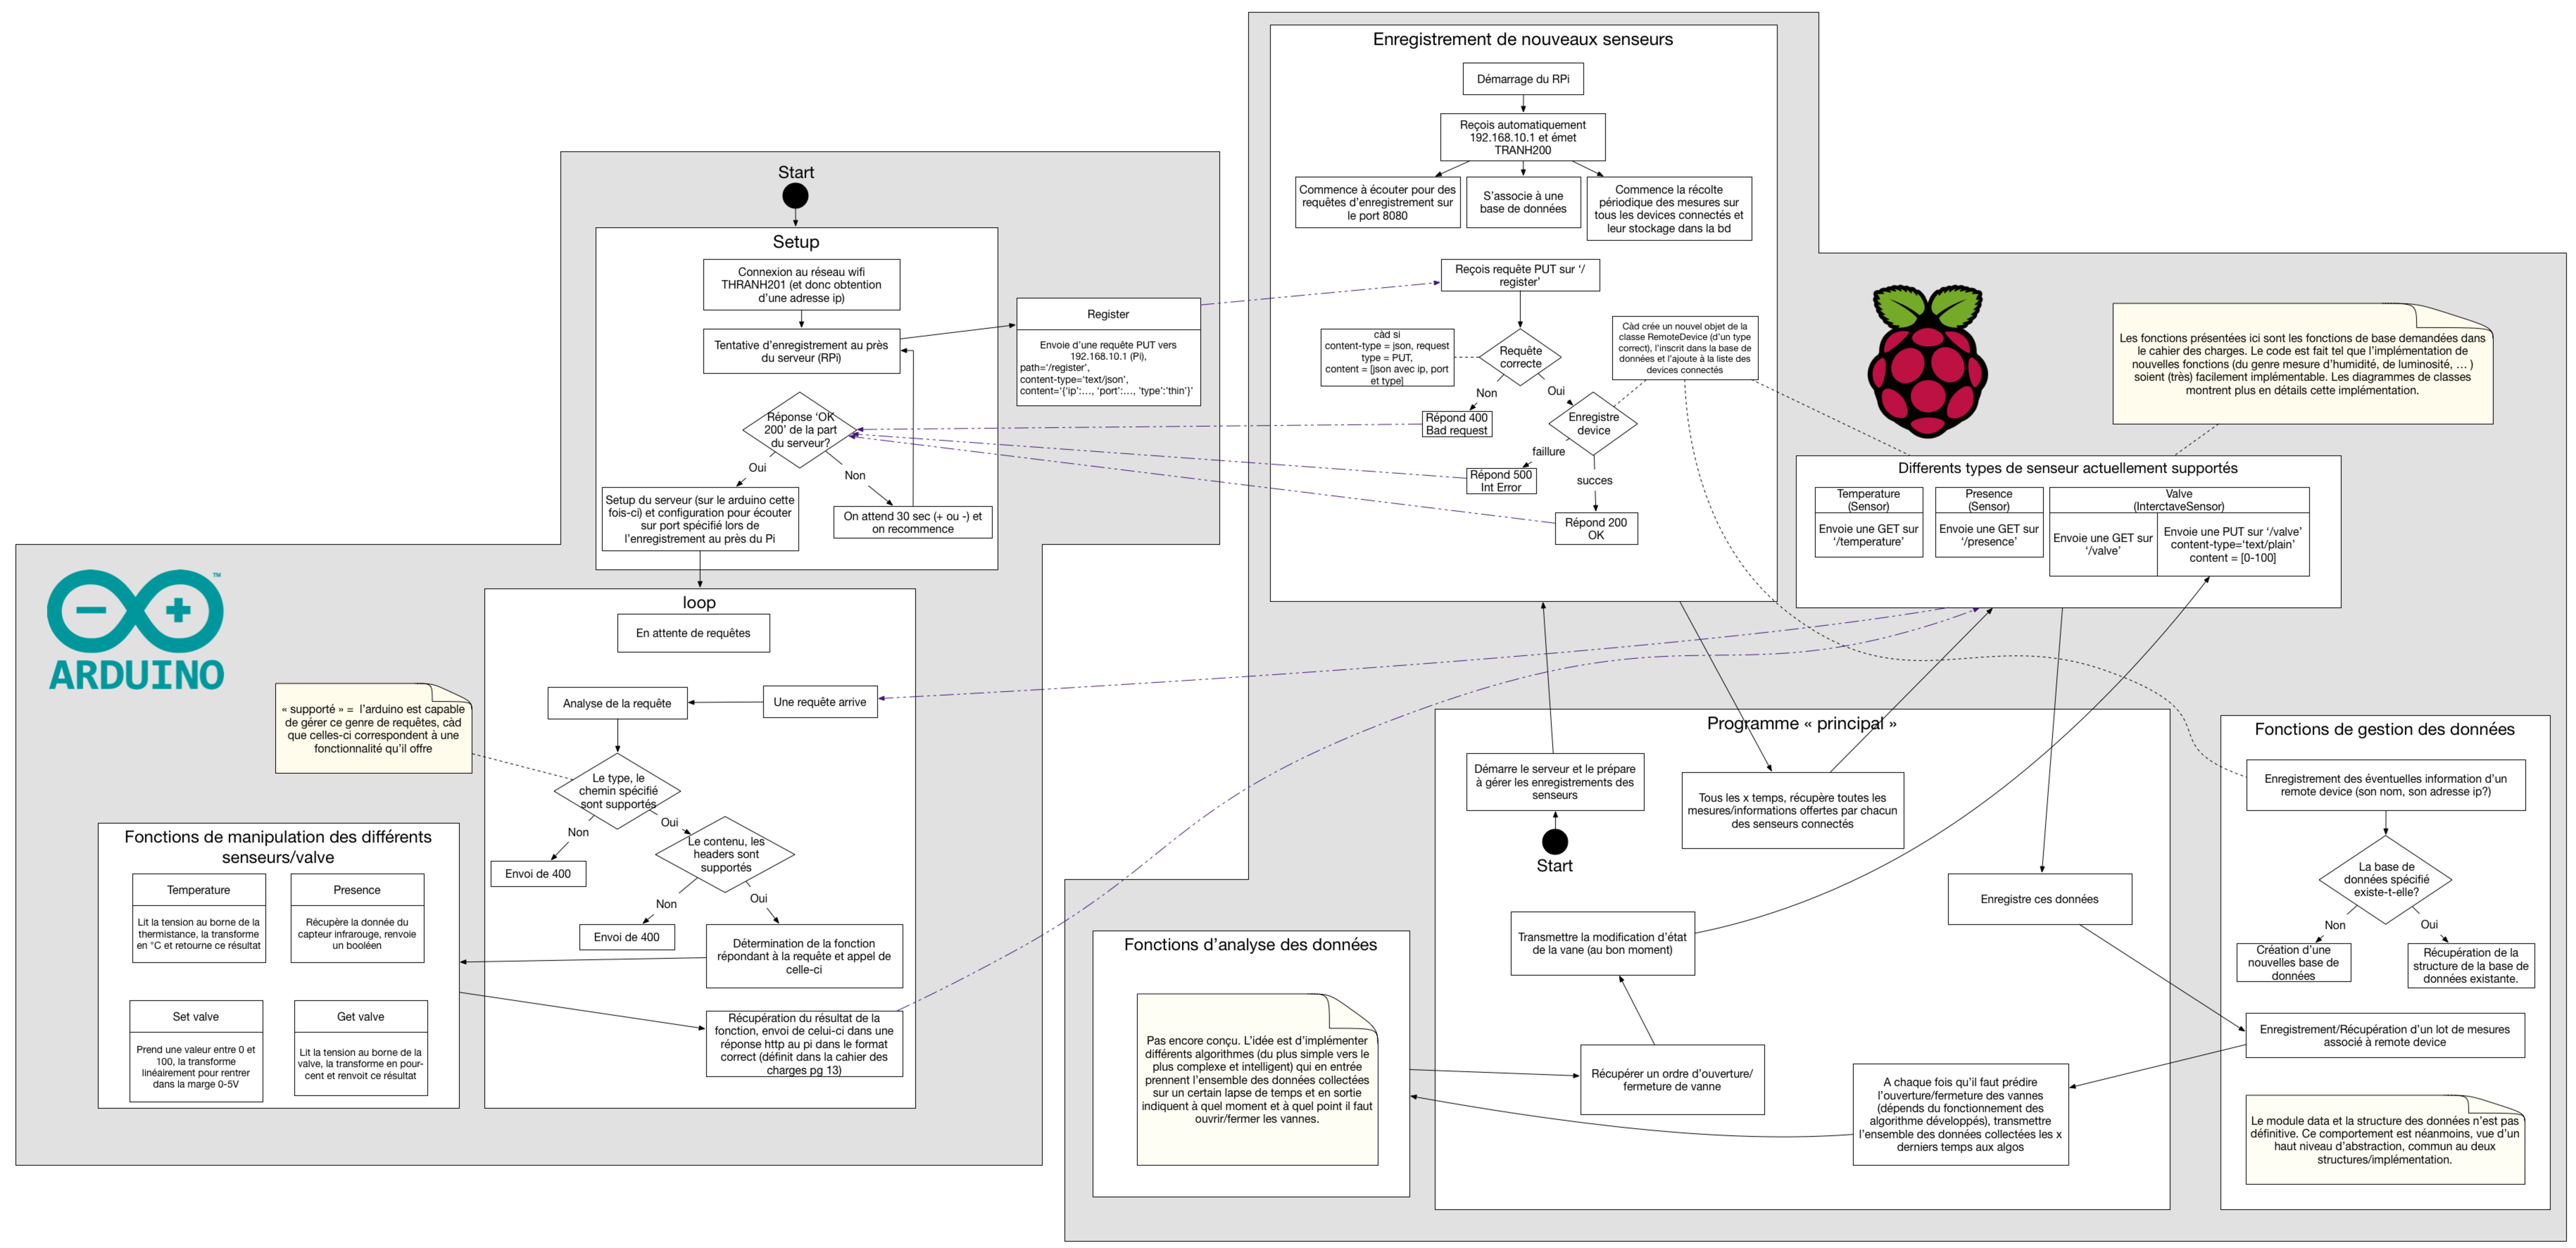
\includepdf[pages={1}, landscape=true, pagecommand=\chapter{Diagramme de comportement global}]{pdf/diagrams_complet.pdf}


\chapter{Diagramme de comportement global}
\label{dia_complet}
Comme expliqué dans la partie Conception, ce diagramme a été créé principalement pour faciliter le travail de groupe. Il offre une vue très synthétique du comportement de l'ensemble du système ainsi que de la façon dont les différentes parties communiquent et interagissent. Il est également disponible sur le Git afin de pouvoir l'utiliser en zoomant dessus.\\

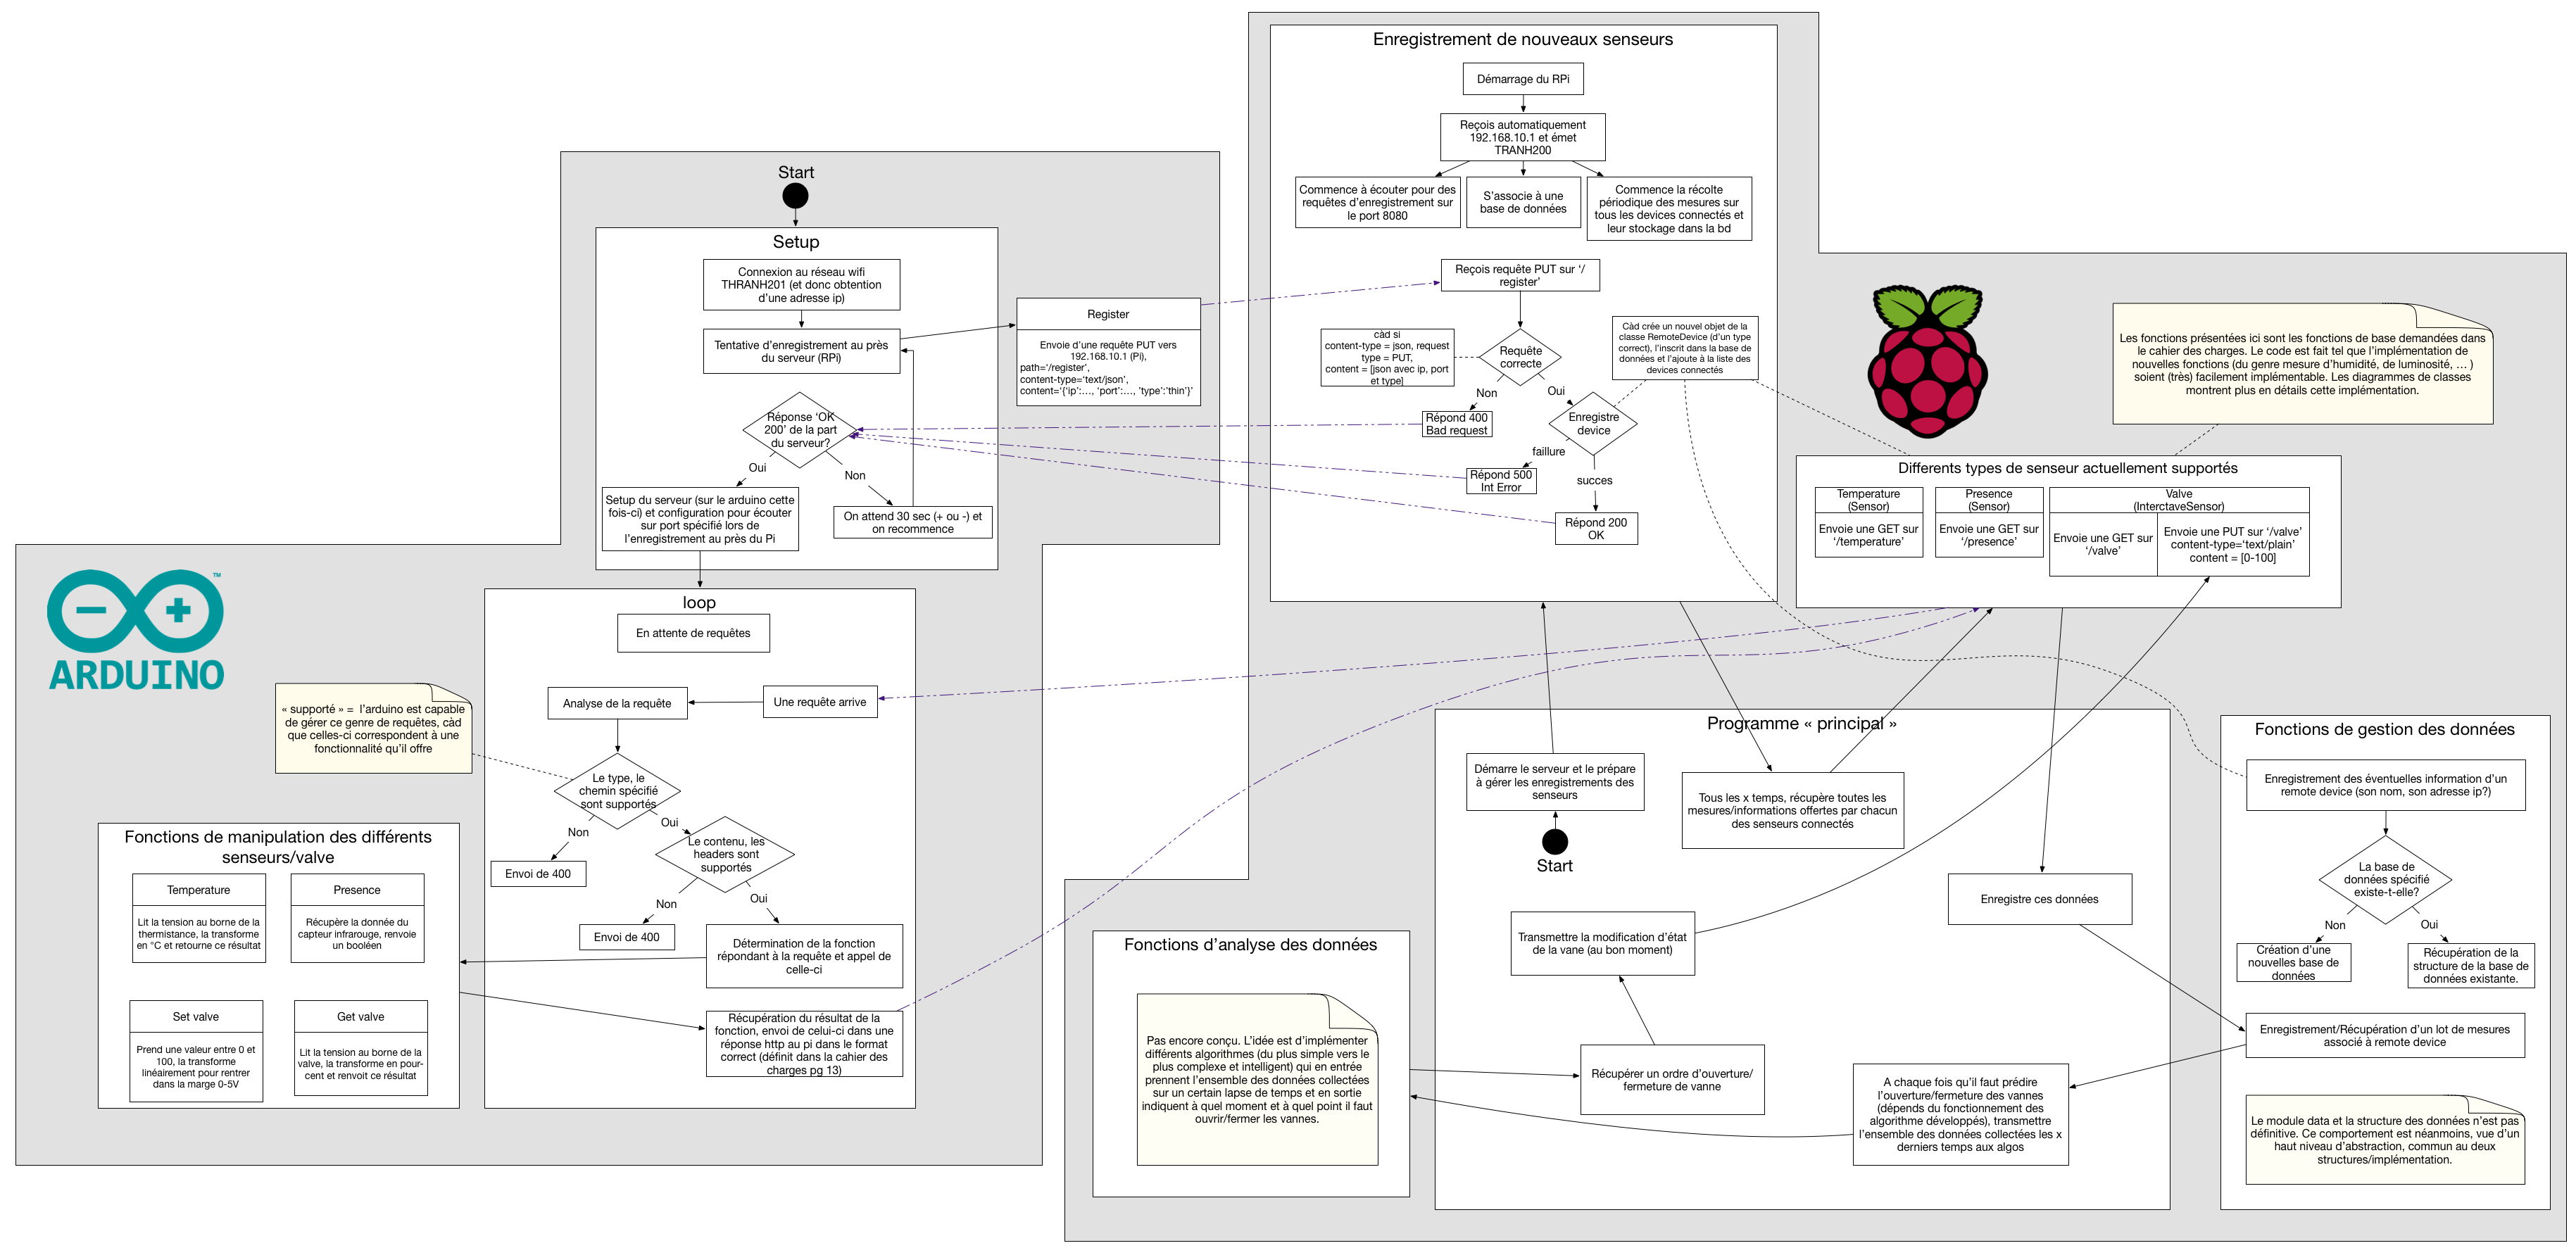
\includegraphics[width=\textwidth]{images/diagrams_complet.png}


% to do : pourquoi 2 fois "chapter"? Regler la lisibilité du schéma qui déborde sur le titre


%--------------------------------------------------------------------------------------
%	CONVENTION DE PROGRAMMATION
%--------------------------------------------------------------------------------------

\chapter{Conventions de programmation}


Dans le but de garder un code propre et maintenable par tous les participants du projet sur le long terme, des conventions et règles de bonne pratique ont été choisies pour être respectées.\\


\section{Code Python}
\begin{itemize}
\item les conventions proposées dans le cours de Thierry Massart \cite{massart}. Notamment pour les docstring, le nommage des classes, des fonctions et des variables,
\item la langue choisie pour le code est l'anglais, pour la simple et bonne raison que c'est la langue universelle des développeurs. Le code n'en est que plus cohérent par rapport aux fonctions prédéfinies.
\item L'orienté objet a été un choix facile : le code n'en est que plus compréhensible, structuré, modulaire et évolutif. 
\item Une attention particulière a été portée à la documentation de chaque méthode/fonction/classe pour éviter une perte de temps à la compréhension et l'analyse du code par les autres membres du groupe et/où par l'auteur lui même dans l'avenir. De cette façon, l'utilisation de ces fonctions est simplifié et ne nécessite que la lecture de la documentation associée pour savoir de quelle façon il faut les appeler et quel type de paramètre il faut leur passer.
\item Les deux modules principaux (\texttt{ThermoServer} et \texttt{Data}) sont accompagnés de diagrammes de classe permettant leur documentation. Ils offrent une vue globale, simplifiée et résumée de leur structure. Cette pratique sera maintenue pour les prochains modules principalement pour son pouvoir documentaire.
\end{itemize}

\section{Code Arduino}

Cette partie a été programmée directement dans le code de base fournis, le style de programmation a donc été calqué sur celui-ci.

%to do : changer les commentaires du code Arduino pour les mettre en anglais..


\newpage

% Il ne faut pas toucher/supprimer ca MERCI :p
% TROP TARD
% CA VA EXPLOSEEEEEEEEER !!!!!
\nocite{int1}
\nocite{int2}
\nocite{int4}
\nocite{int5}
\nocite{int6}
\nocite{int7}
\nocite{int8}
\nocite{ar1}
\nocite{ar2}
\nocite{ar3}
\nocite{ar4}
\nocite{wil1}
\nocite{wil2}
\nocite{wil3}
\nocite{wil4}
\nocite{wil5}
\nocite{s1}
\nocite{s2}
\nocite{pid1}
\nocite{pid2}
\nocite{pid4}
\nocite{pid5}
\nocite{pid6}
\nocite{pid7}
\nocite{ananum}

\bibliography{bibliographie/biblio}
\bibliographystyle{plain} 


\end{document}

